
%----------------------------------------------------------------------------------------
%   PACKAGES AND OTHER DOCUMENT CONFIGURATIONS
%----------------------------------------------------------------------------------------

% latexmk -pvc -pdf
\documentclass[10pt, a4paper, singlespacing]{report}
\usepackage[margin=0.6in]{geometry}
\usepackage{amsmath,amsthm,amsfonts,amssymb}
\usepackage{mathrsfs}
\usepackage{mathtools}
\usepackage{dsfont}
\usepackage[font=scriptsize,labelfont=bf]{caption}
\usepackage[english]{babel}
\usepackage{graphicx}
\newenvironment{Figure}
    {\par\medskip\noindent\minipage{\linewidth}}
    {\endminipage\par\medskip}
\usepackage{blindtext}

% Colours:
\usepackage[table]{xcolor}
\definecolor{purple}{RGB}{117,77,226}

% Hyperlinked references, contents:
\usepackage[bookmarksopen,
  pagebackref,
  % pdfpagelayout=TwoPageRight,
  colorlinks=true,
  urlcolor=purple,
  citecolor=purple,
  filecolor=purple,
  linkcolor=purple,
  linktocpage=true]
  {hyperref}

%----------------------------------------------------------------------------------------
%   TITLE PAGE
%----------------------------------------------------------------------------------------

\begin{document}
\begin{titlepage}
\begin{center}

\vspace{0.5cm}
\textsc{PHS3360 - Physics Project Report} \\
\vspace{2.5cm}

{\Huge Simulating phase contrast imaging for materials with variable density}
\vspace{3cm}

{\LARGE Ana Fabela Hinojosa \footnote{acfab1@student.monash.edu.au}} \\
\vspace{0.4cm}
{\Large Supervisor:\\ Assoc. Prof. Marcus Kitchen \\}
\textsc{School of Physics \& Astronomy} \\
\vspace{3cm}

\includegraphics[scale=0.2]{logo.jpg} \\ % University logo
\vspace{3cm}
{\LARGE November 2021}\\
\vspace{0.5cm}
\end{center}
\end{titlepage}

%----------------------------------------------------------------------------------------
%   QUOTATION PAGE
%----------------------------------------------------------------------------------------

\vspace*{0.2\textheight}

\noindent{``The questions are important. I have thought harder about them than I have about the answers I already have. That is the first thing I know for sure: If the questions don't make sense, neither will the answers.''}\bigbreak

\hfill Kurt Vonnegut.

\vspace{20cm}

%----------------------------------------------------------------------------------------
%   LIST OF CONTENTS/FIGURES/TABLES PAGES
%----------------------------------------------------------------------------------------

\tableofcontents % Prints the main table of contents

\vspace{20cm}

\listoffigures % Prints the list of figures

\vspace{20cm}

% \listoftables % Prints the list of tables


%----------------------------------------------------------------------------------------
%  CONTENTS
%----------------------------------------------------------------------------------------

\begin{abstract}\label{Abstract}
This work studies the theoretical perspective of coherent X-ray imaging. One of the objectives of this project is to determine whether a density difference alone can give phase contrast and, if so, whether the phase contrast is likely to be detected in real experiments. Using simulations of cylinder-shaped sample materials subjected to X-ray wave-fields of different energies, the importance of material density in phase contrast imaging is demonstrated. This report also includes details on an experiment that shows how phase contrast of X-ray imaged objects can be enhanced by decreasing the breath of X-ray polychromatic spectra. Lastly, this work investigates possible improvements to the numerical techniques used in the field of X-ray imaging and presents an improved accuracy method for numerical phase contrast simulations based on the transport-of-intensity equation.
\end{abstract}
%%%%%%%%%%%%%%%%%%%%%%%%%%%%%%%%%%%%%%%%%%%%%%%%%%%%%%%%%%%%%%%%%%%%%%%%%%%%%%%%%%%%%%%%%%%%%%%%%%%%%%%%%%%%%%%%%%%%%%%%%%%%%%%%%%%%%%%%%%%%%%%%%%%%%%%%%%%%%%%%%%%%%%%%%%%%%

\chapter{Introduction}\label{Introduction}
This chapter describes the theoretical background of the field of X-ray optics. Specifically, the mathematical formalism used in phase contrast imaging and in phase retrieval. The origin of X-ray optics lies with Maxwell's classical electrodynamics\cite{PagsTutes}. Since Maxwell's equations describe electromagnetic field disturbances as waves, the spatial and temporal evolution of electromagnetic fields in space can be described by wave optics. Under the wave formalism, there has been substantial progress in the theoretical understanding of the interactions of X-rays with matter, and in the knowledge of how to exploit these interactions experimentally.
%%%%%%%%%%%%%%%%%%%%%%%%%%%%%%%%%%%%%%%%%%%%%%%%%%%%%%%%%%%%%%%%%%%%%%%%%%%%%%%%%%%%%%%%%%%%%%%%%%%%%%%%%%%%%%%%%%%%%%%%%%%%%%%%%%%%%%%%%%%%%%%%%%%%%%%%%%%%%%%%%%%%%%%%%%%%%
\section{X-ray phase contrast imaging}\label{PC}

\subsubsection{Helmholtz equation and the Angular spectrum formulation}\label{ASF}
The Helmholtz equation represents a time-independent form of the wave equation and it is a central equation of diffraction theory\cite{CH49}\cite{Pags2006}.
In general, X-ray imaging is done with polychromatic X-rays with non-trivial spectra\cite{CH49}. It is possible to use a method known as the angular spectrum formulation (ASF) on a wave function in order to greatly simplify radiological imaging. The ASF comprises spectral decomposition of a wave-function into monochromatic components. The separation of each component with an individual fixed angular frequency (i.e. a trivial dependence in time), transforms the wave equation into a time-independent partial differential equation (PDE) that is applied individually to each monochromatic component. After the individual analysis of each component is done, a recombination of the monochromatic components results in the complete description of the polychromatic process\cite{CH49}\cite{Pags2006}.

The complex scalar wave-field function $\Psi(\mathbf{r},t) = \sqrt{I(\mathbf{r},t)} \mathrm{exp}(i \phi(\mathbf{r},t))$ obeys the wave equation in a vacuum
\begin{equation}\label{eq:1}
\left ( \frac{1}{c^2} \frac{\partial^2 }{\partial t^2} -\nabla^2 \right ) \Psi(\mathbf{r},t) = 0,
\end{equation} 
where \textit{c} is the speed of light and $\nabla$ is the Laplacian operator.
The spectral decomposition of $\Psi(\mathbf{r},t)$ is done via the Fourier transform
\begin{equation}\label{eq:2}
\Psi(\mathbf{r},t) = \frac{1}{\sqrt{2 \pi}} \int_{0}^{\infty}\psi_{\omega}(\mathbf{r}) e^{-i\omega t}d\omega,
\end{equation}
notice that the integral only considers a positive integration range (due to analyticity concerns\cite{PagsTutes}). In equation (\ref{eq:2}) the spatial wave-function subscript $\omega$ indicates functional dependence on this quantity\cite{Pags2006}. Evaluating equation (\ref{eq:1}) using equation (\ref{eq:2}) yields the Helmholtz equation for the vacuum
\begin{equation}\label{eq:3}
\left ( \frac{1}{c^2}\frac{\partial^2}{\partial t^{2}} - \nabla^{2}  \right )\Psi(\mathbf{r},t) = 0,
\end{equation}
\begin{equation}\label{eq:4}
\therefore \int_{0}^{\infty} \frac{1}{\sqrt{2 \pi}} \left ( \frac{1}{c^2}\frac{\partial^2}{\partial t^{2}} -\nabla^{2}  \right )  
\psi_{\omega}(\mathbf{r}) e^{-i\omega t}d\omega = 0,
\end{equation}
\begin{equation}\label{eq:5}
\therefore \int_{0}^{\infty} \frac{1}{\sqrt{2 \pi}} \left ( \frac{-\omega^2}{c^2}\psi_{\omega}(\mathbf{r}) e^{-i\omega t} -\nabla^{2}\psi_{\omega}(\mathbf{r}) e^{-i\omega t} \right ) d\omega  
 = 0,
\end{equation}
\begin{equation}\label{eq:6}
\left ( k^2 + \nabla^{2} \right ) \psi_{\omega}(\mathbf{r})  
 = 0,
\end{equation}
where the wave vector $k = \omega/c$.

\subsubsection{Paraxial fields}\label{Paraxial}
In most situations involving phase-contrast imaging, X-ray fields behave as paraxial fields. Electromagnetic (EM) energy in this context is concentrated within a small region about the beam axis. A beam is an EM wave propagating in free space with small divergence (i.e. spread) away from the propagation axis, hence the origin of the name \textit{paraxial}.
In the previous section $\Psi(\mathbf{r},t)$ described a complex scalar wave-field. In this section the paraxiality condition is added to this wave-field.
Under this approximation the complex disturbance $\psi_{\omega}(\mathbf{r})$ present in the Helmholtz equation is expressed as a product of a z-directed plane wave $\mathrm{exp}(ikz)$ and a perturbing envelope $\Phi(\mathbf{r})$\cite{PagsTutes}\cite{CH49}
\begin{equation}\label{eq:7}
\psi_{\omega}(\mathbf{r}) = \Phi(\mathbf{r})\mathrm{exp}(ikz),
\end{equation}
\begin{Figure}
\centering
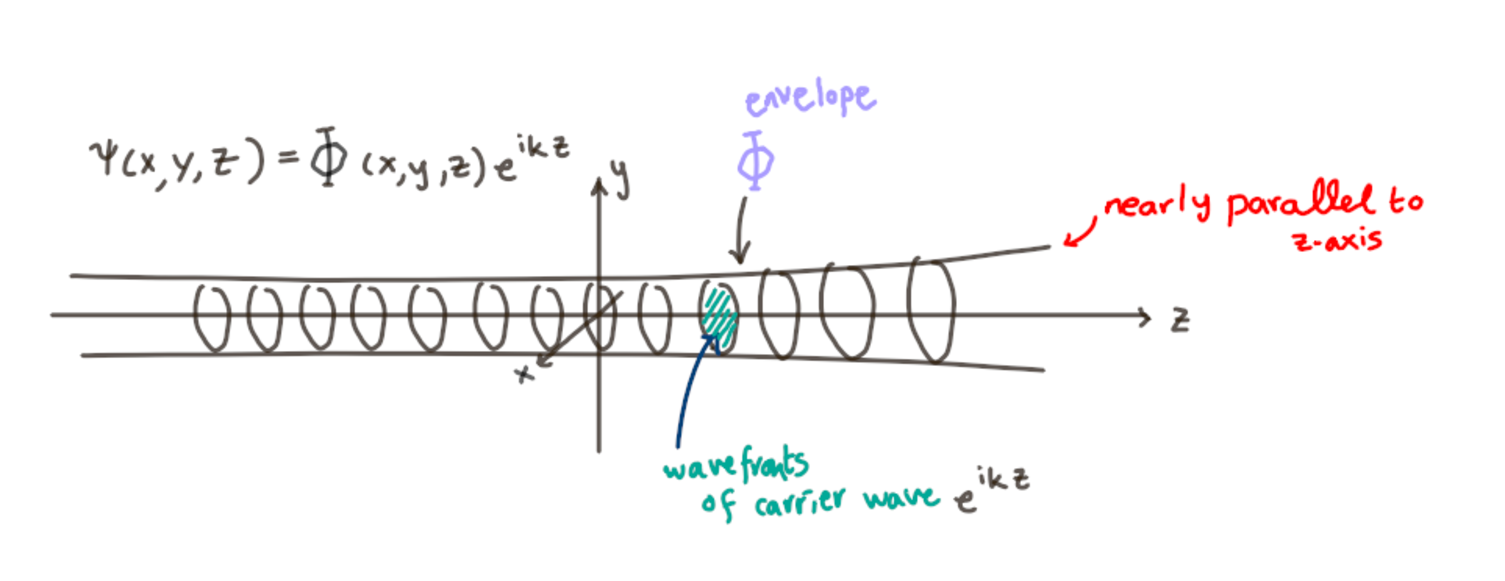
\includegraphics[width=0.6\linewidth]{paraxial_beam.pdf}\label{fig:1}
\captionof{figure}{A cartoon of a paraxial wave-field $\psi_{\omega}(\mathbf{r})$ displaying beam propagation properties along the z-axis. The slowly varying complex envelope is modulated by a carrying plane wave.}
\end{Figure}
the longitudinal variation of the complex envelope $\Delta z = \lambda = 2 \pi/k$ is required to be smaller than the complex envelope itself
\begin{equation}\label{eq:8}
\frac{\Delta \Phi(\mathbf{r})}{\Phi(\mathbf{r})} \leq 1
\end{equation}
using equation (\ref{eq:8}) and the longitudinal variation $\Delta z$  in the Helmholtz equation yields the paraxial Helmholtz equation in the vacuum
\begin{equation}\label{eq:9}
\left (\nabla_{\perp}^{2} + 2 i k \frac{\partial }{\partial z}\right ) \Phi(\mathbf{r}_{\perp}, z) = 0
\end{equation}

\subsubsection{Refractive index and the projection approximation}\label{PA}
In the presence of static, non-magnetic, scattering material media the complex scalar X-ray wave-field can still be studied by using the inhomogeneous Helmholtz equation 
\begin{equation}\label{eq:10}
\left ( k^2 n^2 (\mathbf{r}) + \nabla^{2}  \right )\Psi(\mathbf{r}) = 0,
\end{equation}
where $n(\mathbf{r})$ is the position dependent and complex form for the refractive index, the real part of which corresponds to the refractive index and the imaginary part of this complexified refractive index can be related to the absorptive properties of a sample\cite{PagsTutes}.
\begin{equation}\label{eq:11}
n(\mathbf{r}) = 1 - \delta(\mathbf{r}) + i \beta(\mathbf{r}),
\end{equation}
where $|\delta|, |\beta| << 1$. Using the complex refractive index in the inhomogeneous paraxial Helmholtz equation yields the \textit{projection approximation}, which is an expression that describes the phase shift and attenuation undergone by an X-ray wave moving across a sample
\begin{equation}\label{eq:12}
\Phi(\mathbf{r}_{\perp}, z_0) = \mathrm{exp} \left ( -ik \int_{0}^{z_0}(\delta - i\beta)dz\right ) \Phi(\mathbf{r}_{\perp}, 0)
\end{equation}
\begin{Figure}
\centering
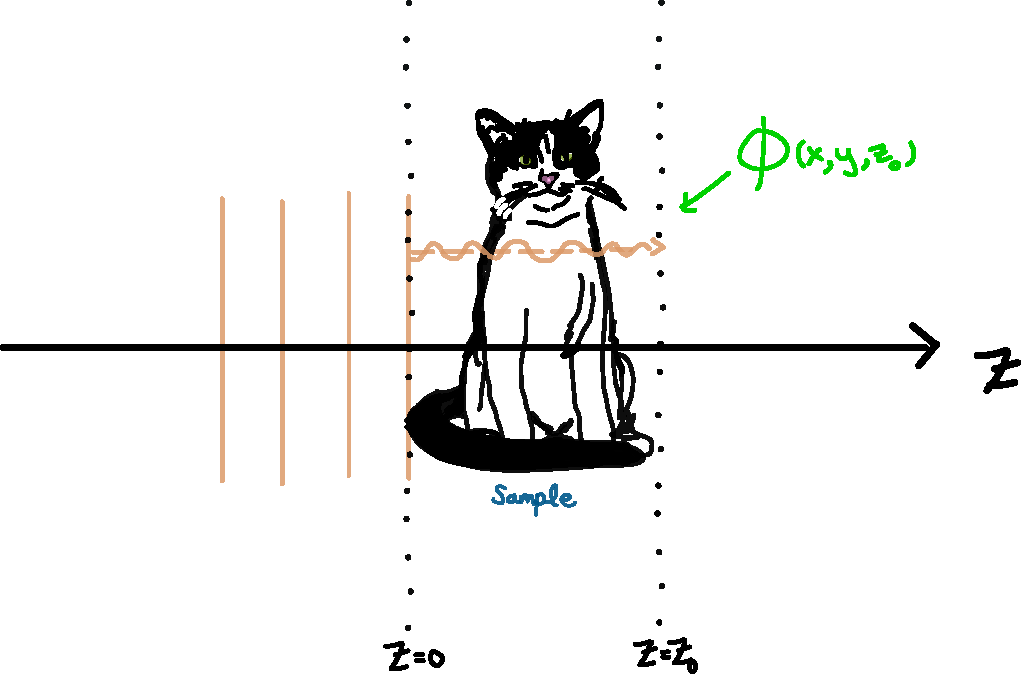
\includegraphics[width=0.6\linewidth]{projection_approximation.pdf}\label{fig:2}
\captionof{figure}{Schematic diagram of the projection approximation adapted from references \cite{CH49} and \cite{Pags2006}. The sample is contained within the space between $z = 0$ and $z = z_0$. The sample is described by its refractive index $n(\mathbf{r})$ which differs from the the refractive index of the air volume that surrounds the sample. In this figure one can see that the path of X-rays passing through an object can be described by defining a surface (also known as the contact plane) immediately downstream from the irradiated object (i.e. $z = z_0$). at which the transferred transverse intensity and phase changes of the incident X-rays are imprinted\cite{CH49}. }
\end{Figure}

The projection approximation assumes that X-ray flow may be well approximated by straight lines parallel to z\cite{PagsTutes} and that most X-rays passing through an object do not actually interact with the sample material (i.e. minimal to no scattering occurs within the sample, a fair assumption due to small magnitude of the complex \textit{refractive index} of X-rays). Neglecting scattering effects is mathematically equivalent to discarding the transverse Laplacian term in equation (\ref{eq:9})\cite{CH49}, in addition, when X-ray--matter interaction are considered then we utilise the inhomogeneous paraxial Helmholtz equation
\begin{equation}\label{eq:13}
\left ( 2 i \frac{\partial }{\partial z} + k ( n^2 (\mathbf{r}) - 1 )\right ) \Phi(\mathbf{r}) = 0.
\end{equation}

\subsubsection{Intensity and phase-shift}\label{Intensity and phase}
Refraction is a property that may be augmented by the intensity attenuation due to the imaged object. This latter quantity may be obtained by taking the squared
modulus of equation (\ref{eq:12}), to give the \textit{Beer-Lambert law}\cite{PagsTutes}
\begin{equation}\label{eq:14}
I(\mathbf{r}_{\perp}, z = z_0) = I^{\mathrm{in}} e^{-\mu T(\mathbf{r}_{\perp})},
\end{equation}
where $T(\mathbf{r}_{\perp})$ is the projected thickness of the object in the direction of the beam propagation, and, $I^{\mathrm{in}}$ the incident light intensity to the object. This expression is also known as the ``contact image ". Equation (\ref{eq:14}) relates the imaginary part of the refractive index $\beta$ to the \textit{linear attenuation coefficient} $\mu = 2k\beta$. 
Since we are working with a wave picture, refraction is associated with wave-front deformation rather than ray deflection, therefore the projection approximation term involving the refractive index $\delta$ (refractive properties of the sample), quantifies the deformation of the X-ray wave-fronts due to passage through the sample. Physically, for each fixed transverse coordinate $(x, y)$, phase-shifts (and the associated wave-front deformations) are continuously accumulated along energy-flow streamlines\cite{PagsTutes}.
\begin{equation}\label{eq:15}
\Delta \phi(\mathbf{r}_{\perp}) = -k \delta T(\mathbf{r}_{\perp}),
\end{equation}
where $k$ is the X-ray wave-number, and $\delta$ the refractive index decrement.

\subsubsection{Transport-of-intensity equation}\label{TIE}
The transport-of-intensity equation (TIE) expresses the intensity and phase evolution of a paraxial monochromatic scalar electromagnetic or matter wave on propagation\cite{Pags2002}. The TIE is also used to quantify the contrast (i.e. refractive (phase) effects) present in propagation-based X-ray phase contrast images\cite{PagsTutes}.
More concisely, the TIE physically describes the change in the light intensity (eq.\ref{eq:14}) and phase (eq.\ref{eq:15}) as the divergence of the transverse energy-flow vector known as the Poynting vector $(\textbf{S})$. If the divergence of this vector is positive, (i.e. the wave-field is locally expanding), optical energy moves away from the local optic axis and so the longitudinal derivative of
intensity will be negative. The converse occurs if the divergence of the Poynting vector is negative, and so the longitudinal derivative of intensity will be positive\cite{PagsTutes}.
\begin{equation}\label{eq:16}
-\nabla_{\perp} \cdot [I(\mathbf{r}) \nabla_{\perp} \phi(\mathbf{r})] = k \frac{\partial I (\mathbf{r})}{\partial z}.
\end{equation}
where $k$ is the wave-number, $I(\mathbf{r})$ is the intensity and $\phi(\mathbf{r})$ is the phase of the X-ray beam, the Poynting vector $\textbf{S} \propto I(\mathbf{r}) \nabla_{\perp} \phi(\mathbf{r})$.

%%%%%%%%%%%%%%%%%%%%%%%%%%%%%%%%%%%%%%%%%%%%%%%%%%%%%%%%%%%%%%%%%%%%%%%%%%%%%%%%%%%%%%%%%%%%%%%%%%%%%%%%%%%%%%%%%%%%%%%%%%%%%%%%%%%%%%%%%%%%%%%%%%%%%%%%%%%%%%%%%%%%%%%%%%%%%
\section{X-ray phase retrieval}\label{PR}
Decoding of X-ray phase contrast images is essentially the reverse problem to phase contrast imaging and it is known as \textit{phase retrieval}. 
In general inverse problems are more complex than forward problems. Often inverse problems are unsolvable, and, even if there exist possible solutions to these problems, these may not be unique or stable with regards to realistic experimental conditions. 
Phase retrieval seeks to reconstruct both the intensity and phase of the input field, given only the intensity of the output field of the imaging system\cite{PagsTutes}\cite{Pags2002}. Under the projection approximation (described in section \ref{PA}), it is clear that both the intensity (\ref{eq:14}) and the phase (\ref{eq:15}) on the contact plane (Figure \ref{fig:2}) are both described by the projected thickness ($T(\mathbf{r}_{\perp})$) of the sample object. Paganin et al.(2002) developed a fast and deterministic method for quantitative phase extraction\cite{Pags2002} using the TIE to propagate a wave-field's intensity (\ref{eq:14}) and phase (\ref{eq:15}) by a sufficiently small distance away from the sample.
Substituting the contact plane intensity and phase of the illuminating beam at the contact plane into equation (\ref{eq:16}) returns a non linear equation in $T(\mathbf{r}_{\perp})$
\begin{equation}\label{eq:17}
- \frac{\delta}{\mu} I^{\mathrm{in}} \nabla^{2}_{\perp} e^{-\mu T(\mathbf{r}_{\perp})} = \frac{\partial}{\partial z}I(\mathbf{r}_{\perp}, z=0).
\end{equation}
This phase retrieval method\cite{Pags2002} approximates the right hand side of equation \ref{eq:17} by the first order finite difference formula
\begin{equation}\label{eq:18}
\frac{\partial}{\partial z}I(\mathbf{r}_{\perp}, z=0) \approx \frac{I(\mathbf{r}_{\perp}, z=z_0) - I^{\mathrm{in}} e^{-\mu T(\mathbf{r}_{\perp})}}{z_0},
\end{equation}
replacing equation (\ref{eq:18}) into equation (\ref{eq:16}) and rearranging to find the ratio of the intensity at the detector plane (i.e.the phase contrast image $I(\mathbf{r}_{\perp}, z = z_0)$) to the intensity initially incident to the object
 \begin{equation}\label{eq:19}
\left (\frac{- z_0 \delta}{\mu}\nabla^{2}_{\perp} + 1 \right )e^{-\mu T(\mathbf{r}_{\perp})} = \frac{I(\mathbf{r}_{\perp}, z=z_0)}{I^{\mathrm{in}}}.
\end{equation}
The construction of the phase retrieval algorithm requires that the contact image and the phase contrast image are represented as Fourier integrals\cite{Pags2002}
\begin{align}\label{eq:20}
&I^{\mathrm{in}} e^{-\mu T(\mathbf{r}_{\perp})} = \frac{I^{\mathrm{in}}}{2 \pi} \int \int \mathscr{F} \left \{ e^{-\mu T(\mathbf{r}_{\perp})} \right \} e^{i \mathbf{k}_{\perp}\cdot \mathbf{r}_{\perp}} d \mathbf{k}_{\perp}
\\&I(\mathbf{r}_{\perp}, z=z_0) = \frac{1}{2 \pi}  \int \int \mathscr{F} \left \{ I (\mathbf{r}_{\perp}, z = z_0) \right \} e^{i \mathbf{k}_{\perp}\cdot \mathbf{r}_{\perp}} d \mathbf{k}_{\perp}
\end{align}
where $\mathscr{F}\left \{ \right \}$ represents Fourier transformation. Substituting these equations in equation (\ref{eq:19})
\begin{equation}\label{eq:21}
\mathscr{F}\left \{ e^{-\mu T(\mathbf{r}_{\perp}} \right \} = \mu \frac{\mathscr{F}\left \{ I(\mathbf{r}_{\perp}, z=z_0)\right \}/I^{\mathrm{in}}}{z_0 \delta |\mathbf{k}_{\perp}|^{2} + \mu}.
\end{equation}
Taking the inverse Fourier transform of equation (\ref{eq:21}) and solving for $T(\mathbf{r}_{\perp})$
\begin{equation}\label{eq:22}
T(\mathbf{r}_{\perp}) = - \frac{1}{\mu} \mathrm{log}_{e} \left ( \mathscr{F}^{-1} \left \{ \mu \frac{ \mathscr{F} \left \{I(\mathbf{r}_{\perp}, z=z_0) \right \} /  I^{\mathrm{in}}}{z_0 \delta |\mathbf{k}_{\perp}|^{2} + \mu}  \right \} \right ).
\end{equation}
The derivation of this algorithm requires the use of the Fresnel diffraction integral to show that the intensity downstream from a weakly refracting object, is related to the intensity at infinity $I_{\infty}$ and the magnification resultant from using collimated illumination\cite{Pags2002}.
\begin{equation}\label{eq:23}
I_{\mathrm{R_{1}}}(\mathbf{r_{\perp}}, z) = \frac{1}{M^2} I_{\infty} \left ( \frac{\mathbf{r_\perp}}{M}, \frac{z}{M} \right ),
\end{equation}
where $M$ is the image magnification obtained from point source illumination. With equation \ref{eq:23}, equation \ref{eq:22} can be transformed into a form that suits point source illumination\cite{Pags2002}
\begin{equation}\label{eq:24}
T(\mathbf{r}_{\perp}) = - \frac{1}{\mu} \mathrm{log}_{e} \left ( \mathscr{F}^{-1} \left \{ \mu \frac{ \mathscr{F} \left \{M^2 I(M\mathbf{r}_{\perp}, z=z_0) \right \} /  I^{\mathrm{in}}}{z_0 \delta |\mathbf{k}_{\perp}|^{2}/M + \mu}  \right \} \right ).
\end{equation}
this projected thickness is related to the intensity and phase of the radiation at the exit surface of the sample of interest (i.e. the projected thickness of a homogeneous material sample is obtained from a single propagation-based phase contrast image).
In simple terms, the Paganin et al. (2002) algorithm can be thought as bringing into focus the physically defocused images that are obtained using point-projection imaging\cite{Pags2002}.
It is important to remark that information on the properties of objects may be lost on the images obtained with X-rays. Even though X-ray imaging has strong dependence on material density and thickness\cite{CH49}, the projection approximation fails to disambiguate between these two parameters, and this issue can in some instances result in an incomplete description of the imaged material.
%%%%%%%%%%%%%%%%%%%%%%%%%%%%%%%%%%%%%%%%%%%%%%%%%%%%%%%%%%%%%%%%%%%%%%%%%%%%%%%%%%%%%%%%%%%%%%%%%%%%%%%%%%%%%%%%%%%%%%%%%%%%%%%%%%%%%%%%%%%%%%%%%%%%%%%%%%%%%%%%%%%%%%%%%%%%%
\section{X-ray polychromatic spectra}\label{poly}
As explained in section \ref{ASF}, X-ray imaging is done with polychromatic X-rays with non-trivial spectra\cite{CH49}
X-rays are commonly produced by a phenomenon known as X-ray florescence (XRF). A heated filament emits electrons by thermionic emission, these electrons are accelerated by a high voltage and collide with a metal target. In simple terms, the accelerated electrons interact with the atoms comprising the metal target by (i) impacting a shell electron in the target and dislodging it causing photoelectron emission, (ii) having their path deviated without having any actual contact with the target atoms, (iii) directly impacting the nucleus.

Characteristic X-rays are created by the first interaction described above. As the incident electron releases an inner shell electron, this leaves a vacancy in the atom's inner shell. The vacancy is quickly filled by an outer shell electron which causes photon emission with an energy equal to the energy difference between the inner and outer shells. The term ``characteristic" refers to the fact that each element has a distinct pattern of X-ray photoelectron emission.
The second interaction described above is known as Bremsstrahlung (Background/ Breaking) radiation. A source of Bremsstrahlung radiation occurs due to incident electrons interacting with the nuclear electric field. The electron paths may be deflected or decelerated and recaptured by the atom into an energy electron shell. 
\begin{Figure}
\centering
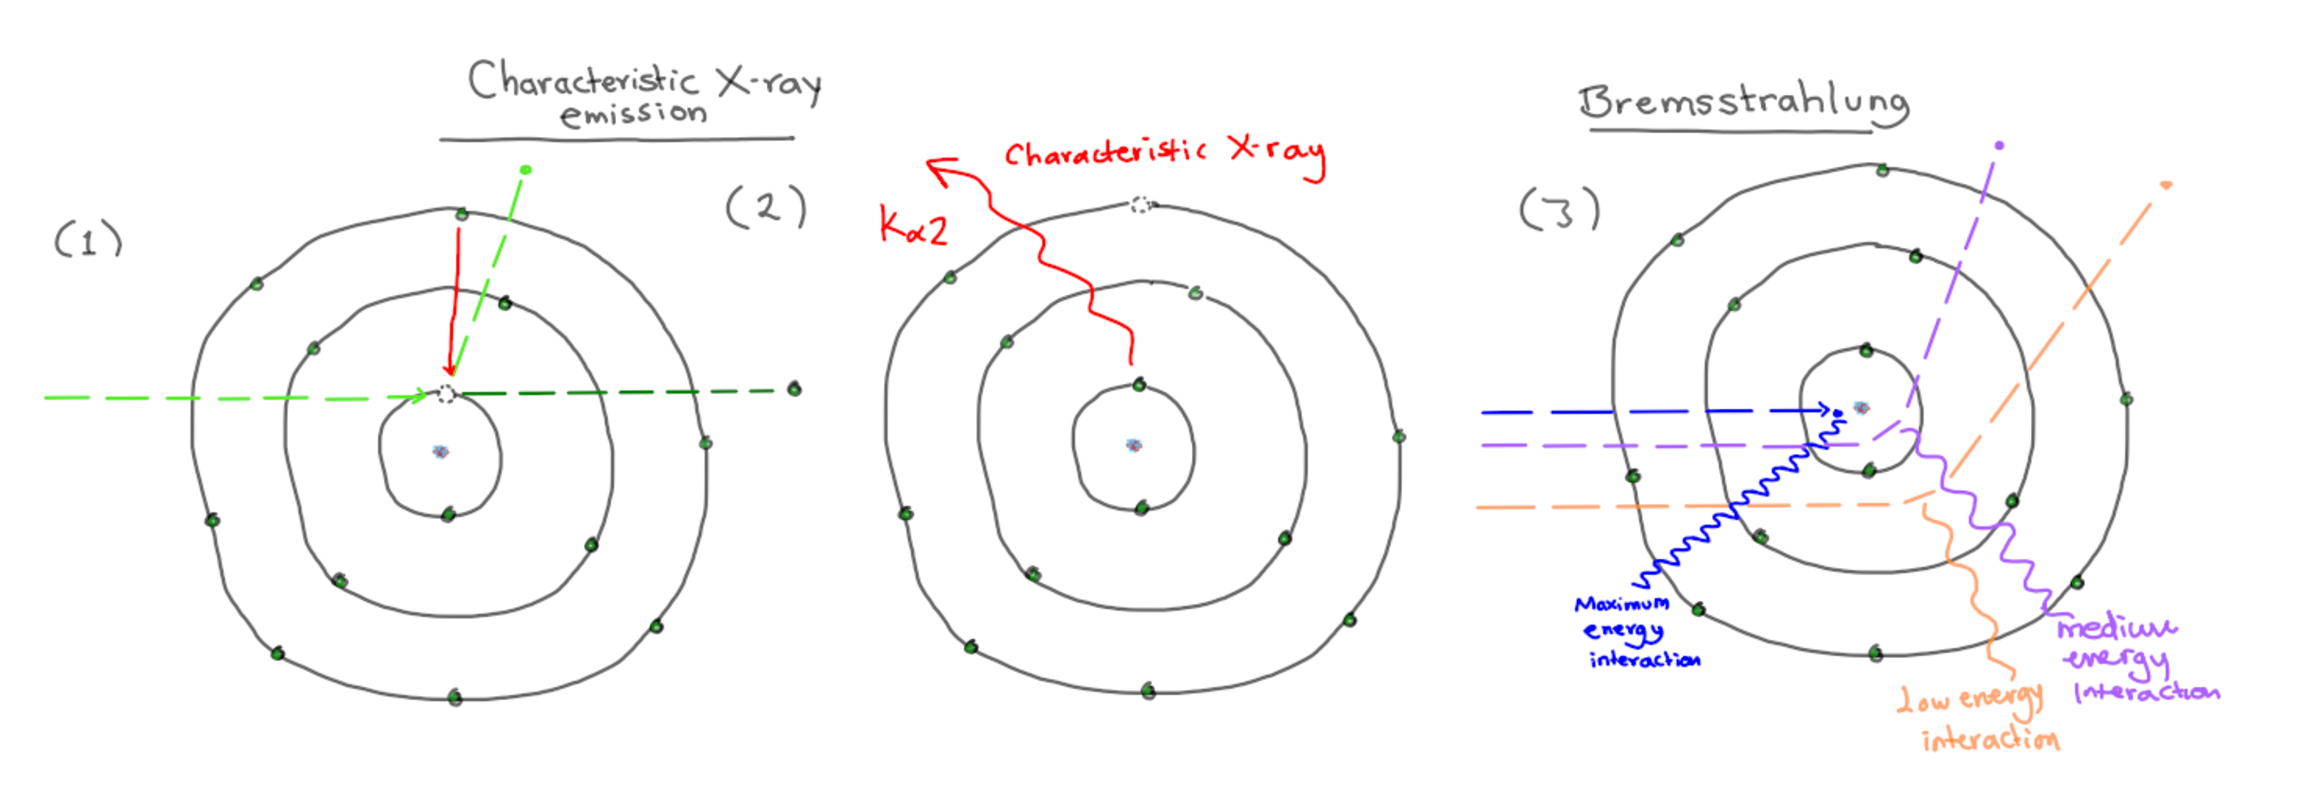
\includegraphics[width=\linewidth]{characteristic_Bremsstrahlung.pdf}\label{fig:3}
\captionof{figure}{Cartoons of accelerated electrons interacting with target atoms. On the left two cartoons (i.e. sub-figures: (1) and (2)), characteristic X-ray emission is represented by (1) an accelerated electron hitting an inner shell electron expelling it from the atom, while an outer shell electron promptly moves inward to fill the inner shell gap (2)releasing the characteristic X-ray. sub-figure: (3) represents a visualisation of the types of possible Bremsstrahlung radiation, ranging from low energy/distant, to high energy interactions between the incident accelerated electrons and the atomic nucleus.}
\end{Figure}
\begin{Figure}
\centering
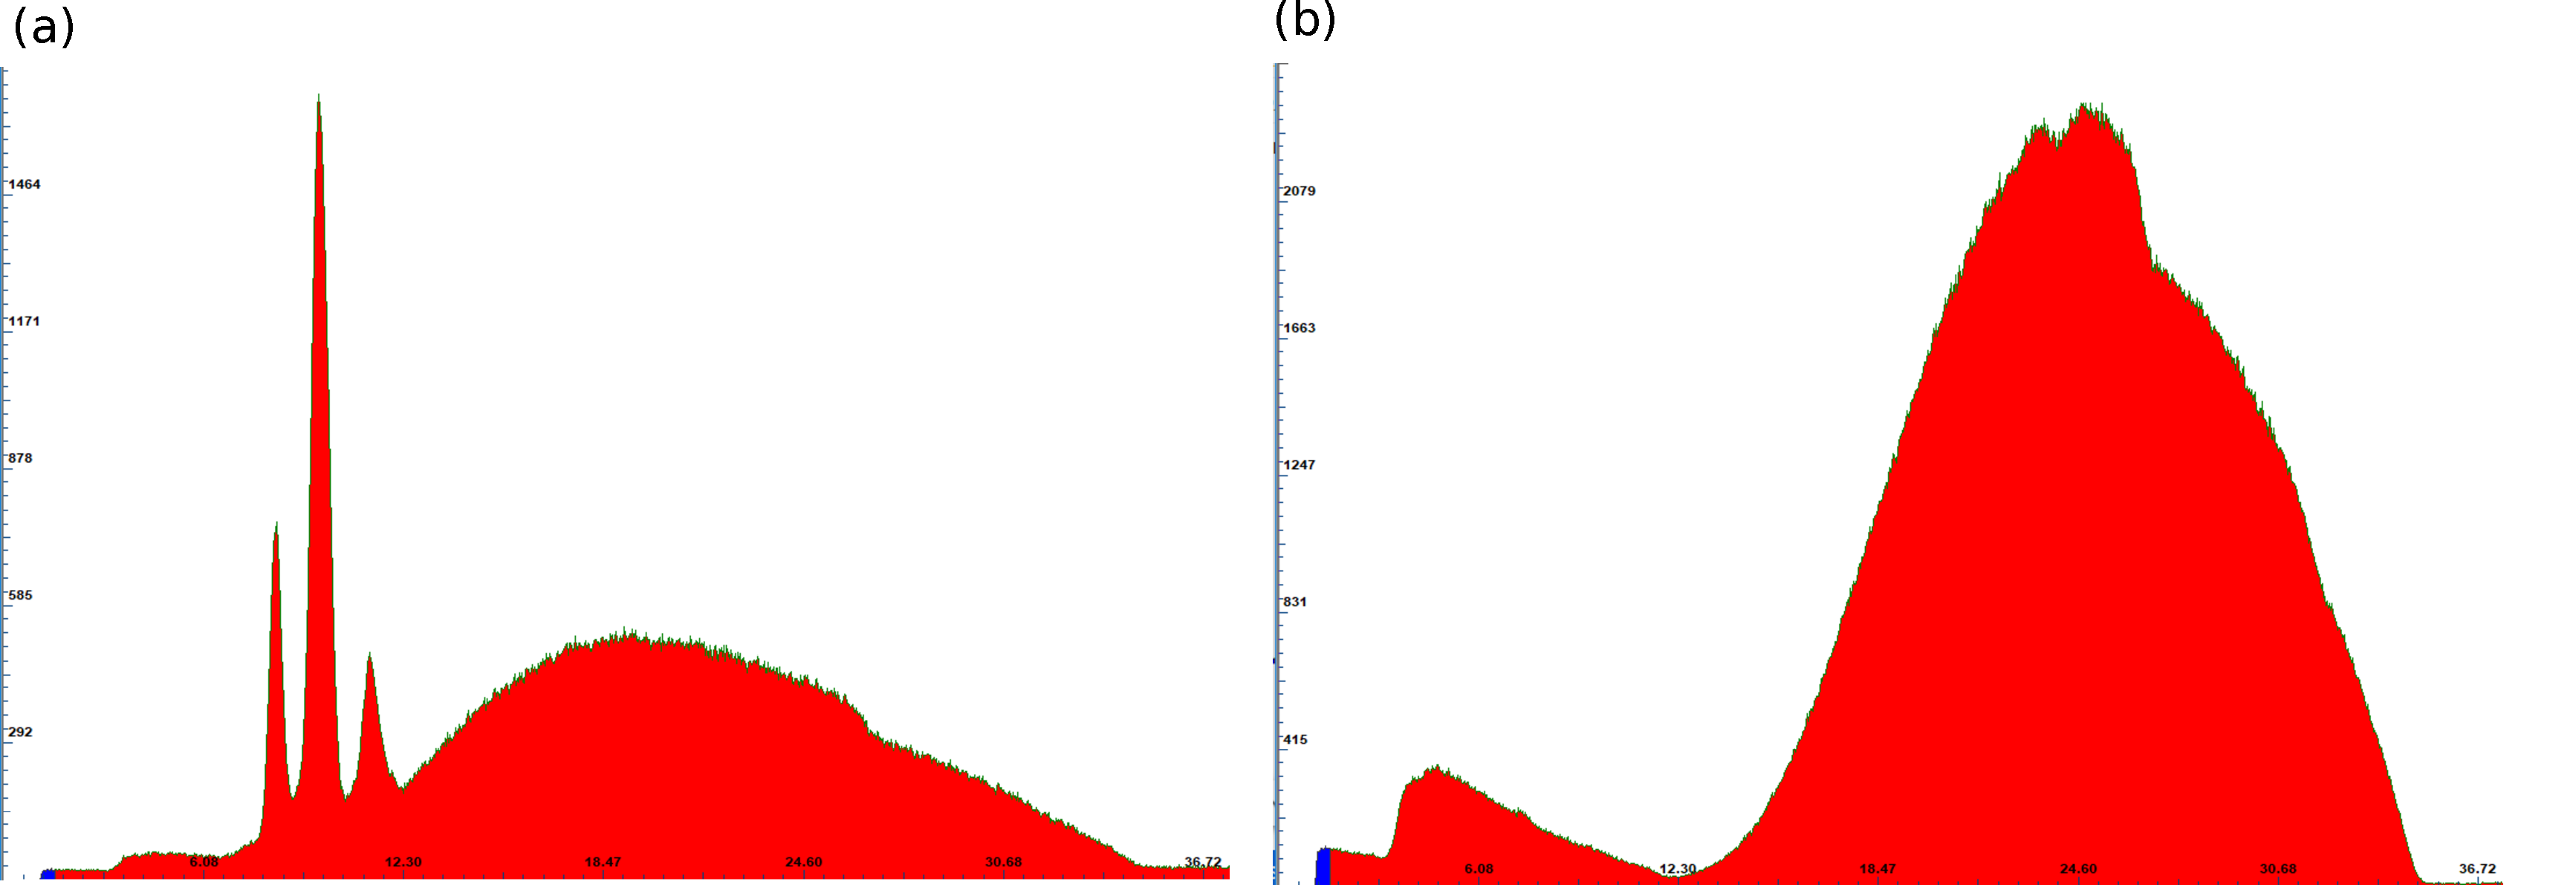
\includegraphics[width=\linewidth]{W_poly_spectrum.pdf}\label{fig:poly}
\captionof{figure}{Original image by M Kitchen (2021). Histograms of photon counts versus energy for the polychromatic spectrum of the tungsten target used in the Monash X-ray imaging laboratory. The energy spread for both sub-figures (a) and (b) is approximately $35$ kV, sub-figure (a) is an unfiltered spectrum while sub-figure (b) was filtered with a piece of Aluminium of thickness $0.5$ mm. In the lower energy region of sub-figure (a), three characteristic X-ray peaks can be seen, these energy peaks are approximately centred at $8.1$ kV, $9.7$ kV and $11.2$ kV from left to right. The Bremsstrahlung peak coloured in red, is centred at approximately $21$ kV. In the case of sub-figure (b) the filtered spectrum aims to simulate a monochromatic energy peak. This peak is approximately centred at $24.6$ kV. in the lower energy region, a smaller undesirable peak is centred approximately at $6$ kV.}
\end{Figure}

Some simulations in this work used selected energy values visible in figure \ref{fig:poly} (i.e. the three characteristic peaks and the Bremsstrahlung peak of tungsten)to quantify potential fringe shifting due to energy dispersion (see section \ref{poly}).
%%%%%%%%%%%%%%%%%%%%%%%%%%%%%%%%%%%%%%%%%%%%%%%%%%%%%%%%%%%%%%%%%%%%%%%%%%%%%%%%%%%%%%%%%%%%%%%%%%%%%%%%%%%%%%%%%%%%%%%%%%%%%%%%%%%%%%%%%%%%%%%%%%%%%%%%%%%%%%%%%%%%%%%%%%%%%

\chapter{Simulations}\label{Simulations}
To determine whether density differences contribute to phase contrast and if so, whether this contribution is actually detectable in a real experiment, I created several simulations of cylinder-shaped sample materials and subjected these samples to X-ray wave-fields of different energies. In some of my simulations, I use a single cylinder made of a homogeneous material. In others I use two embedded concentric cylinder-shaped samples of materials with either an equal chemical composition and different densities or, different chemical compositions, and densities. With these simulations I demonstrate the importance of material density in phase contrast imaging,  by 1) showing how distinctly, phase contrast arises between material boundaries and 2) whether the observed phase contrast is density-dependent. 
I also present the details on my investigations on the undesirable effects produced by the use of X-ray polychromatic spectra in X-ray phase contrast imaging.
These investigations are numerical and experimental. I show below how X-ray phase contrast of imaged objects can be enhanced by narrowing the breath of X-ray polychromatic spectra.
Finally, I describe below an improved accuracy method for numerical phase contrast simulations based on the transport-of-intensity equation using a higher order derivative approximation algorithm known as Runge-Kutta.

%%%%%%%%%%%%%%%%%%%%%%%%%%%%%%%%%%%%%%%%%%%%%%%%%%%%%%%%%%%%%%%%%%%%%%%%%%%%%%%%%%%%%%%%%%%%%%%%%%%%%%%%%%%%%%%%%%%%%%%%%%%%%%%%%%%%%%%%%%%%%%%%%%%%%%%%%%%%%%%%%%%%%%%%%%%%%
\section{Methods}\label{Methods}
For the single cylinder simulations I use the projection approximation to solve the transport-of-intensity equation (TIE). The TIE produces observable changes onto the intensity (\ref{eq:14}) and phase (\ref{eq:15}) when these are used as initial conditions in the propagation problem. For the two-cylinder simulations, I also use the projection approximation, but this time I model the propagation of the monochromatic X-ray wave-field using the angular spectrum formulation (ASF) (section \ref{ASF}). The ASF uses Fourier decomposition of wave-fields at a single plane into distinct component plane waves. Each plane wave component is propagated through the Fourier domain to a destination plane, and then the propagated wave-field components are reconstructed via an inverse spatial Fourier transform\cite{Goodman}. To implement the ASF, I use the X-ray imaging XRI library, since the existing algorithm has already implemented several fixes to undesirable instabilities that can appear in the simulations. The XRI library was built by the Monash X-ray imaging group.

%%%%%%%%%%%%%%%%%%%%%%%%%%%%%%%%%%%%%%%%%%%%%%%%%%%%%%%%%%%%%%%%%%%%%%%%%%%%%%%%%%%%%%%%%%%%%%%%%%%%%%%%%%%%%%%%%%%%%%%%%%%%%%%%%%%%%%%%%%%%%%%%%%%%%%%%%%%%%%%%%%%%%%%%%%%%%
\subsection{Simulating a single homogeneous cylinder}\label{Single cylinder}
I solve the TIE in two-dimensions using the projection approximation to establish my initial conditions.  Originally, my code discretises a two-dimensional space as an array with dimensions $x, y = 1024, 512$. I first attempt to solve the TIE in Fourier space. To calculate the wave-field's derivative terms in equation (\ref{eq:16}), I use the Fourier derivative theorem to write the derivatives. I define functions describing the geometry and, optical properties (i.e. refractive index: $\delta(x, y, z)$ and $\mu(x, y, z)$) of the simulated cylinder. Both $\delta$ and $\mu$ functions use a sigmoid function with adjustable gradient to slightly blur the edge of the cylinder and, avoid instability while calculating the intensity (\ref{eq:14}) and phase (\ref{eq:15}). This method is slow due to the Fourier derivatives, and the output intensity profile after propagation does not appear very stable as several oscillations can be seen in figure \ref{fig:5}. To fix the instability issue, I adjusted the ratio of the spacings in my discretised space several times to make sure that the Nyquist mode of the TIE was resolved adequately. Nevertheless I was unable to obtain a completely smooth, and realistic looking intensity profile in figure \ref{fig:5}.

To complement this investigation, I solved the TIE in position space using finite differences (see figure \ref{fig:6}). In this method I use \texttt{numpy.gradient} to evaluate each derivative and \texttt{scipy.ndimage.laplace} to evaluate the phase Laplacian term in the TIE. This time my code discretised the two-dimensional space as a 2D array $x, y = 1024, 1024$. 

%%%%%%%%%%%%%%%%%%%%%%%%%%%%%%%%%%%%%%%%%%%%%%%%%%%%%%%%%%%%%%%%%%%%%%%%%%%%%%%%%%%%%%%%%%%%%%%%%%%%%%%%%%%%%%%%%%%%%%%%%%%%%%%%%%%%%%%%%%%%%%%%%%%%%%%%%%%%%%%%%%%%%%%%%%%%

\subsection{Simulating two concentric homogeneous cylinders}\label{2 cylinders}
I simulate two concentric cylinders made of two different homogeneous materials using the angular spectrum formulation (ASF) propagation algorithm in the xri library. 
To find the optical parameters of the sample materials (i.e. $\delta$ and $\mu$) under certain energy X-rays, I use the X-ray imaging group ``X-ray attenuation calculator" which employs the values recorded in NIST in database 66: X-Ray Form Factor, Attenuation, and Scattering Tables\cite{NIST}. The ``X-ray attenuation calculator" makes these values easily accessible via a GUI.
I define a function for the projected thickness of the sample cylinders. The thickness function uses an adjustable width Gaussian filter to slightly blur the edge of each cylinder and, avoid instability while calculating the parameters required by the ASF propagation algorithm. The parameters calculated are $\delta T(\mathbf{r}_{\perp})$ and $\beta T(\mathbf{r}_{\perp})$, corresponding to the refraction and absorption parameters respectively. I calculate these quantities for each of the two cylinders in each simulation. Then I combine these quantities because of the concentric feature of the cylinders.

% %%%%%%%%%%%%%%%%%%%%%%%%%%%%%%%%%%%%%%%%%%%%%%%%%%%%%%%%%%%%%%%%%%%%%%%%%%%%%%%%%%%%%%%%%%%%%%%%%%%%%%%%%%%%%%%%%%%%%%%%%%%%%%%%%%%%%%%%%%%%%%%%%%%%%%%%%%%%%%%%%%%%%%%%%%%%%

\subsection{Imaging brain structures}\label{Brainz}
The optical properties of grey and white matter are extremely similar. However, it is known that there is a small difference in the values of the attenuation coefficients of these materials. Computerized tomography (CT) brain imaging has been reported to yield clearly demarcated tissue borders at the grey/white matter boundaries\cite{Beltran2}. To determine if density differences alone produce phase contrast when imaging extremely similar brain materials, I simulated grey and white matter. I use experimental grey and white matter densities reported in the ``IT’IS Database for thermal and electromagnetic parameters of biological tissues" (see reference \cite{ITIS}). I use the X-ray imaging group ``X-ray attenuation calculator" X-Ray Form Factor, Attenuation, and Scattering Tables\cite{NIST} to find the complex refractive index parameters of the whole brain (i.e. $\delta_B$ and $\mu_B$). 

In my second model, I also use the attenuation coefficients for both materials $\mu_{\mathrm{GM}}$ for grey matter, and $\mu_{\mathrm{WM}}$ for white matter. These values were obtained from CT imaging of rabbit and kitten brain samples. The data was acquired at Japan's SPring-8 synchrotron radiation facility using an X-ray energy of $E = 24$keV and a sample-to-detector distance of $5$ m\cite{Linda}.

Using the tools described above, I created two different simulations. I first, calculated an approximate estimate for the grey and white matter refractive index decrements ($\delta_{\mathrm{GM}}$ and $\delta_{\mathrm{WM}}$). In the case of my first simulation, I modelled the refractive index decrements as proportional to the ratio of the attenuation coefficient value for the full brain obtained from reference \cite{NIST} and the density of the grey or white matter values reported in reference \cite{ITIS} (for example for grey matter: $\delta_{\mathrm{GM}} = \frac{\mu_B}{\rho_{\mathrm{GM}}} \delta_B$). In contrast, my second model considered the refractive index decrement to be proportional to the ratio between the attenuation coefficient value for the full brain and the value corresponding to either the grey or white matter attenuation coefficients(for example for grey matter: $\delta_{\mathrm{GM}} = \frac{\mu_B}{\mu_{\mathrm{GM}}} \delta_B$). 

%%%%%%%%%%%%%%%%%%%%%%%%%%%%%%%%%%%%%%%%%%%%%%%%%%%%%%%%%%%%%%%%%%%%%%%%%%%%%%%%%%%%%%%%%%%%%%%%%%%%%%%%%%%%%%%%%%%%%%%%%%%%%%%%%%%%%%%%%%%%%%%%%%%%%%%%%%%%%%%%%%%%%%%%%%%%%

\subsection{The problems with polychromatic spectra}\label{poly}
Given that the mathematical background of phase contrast imaging requires the assumption of wave-field monochromaticity (see \ref{ASF}), this work investigates how phase contrast of X-ray imaged objects can be enhanced by decreasing the range of polychromatic spectra. 
First, I carried out simulations of monochromatic spectra throughout the whole energy range of Tungsten at $35$ kV. The simulations were created using three different methods of propagation based phase contrast, the angular spectrum formulation (ASF) (see \ref{ASF}), the transport-of-intensity equation implemented using fourth order Runge-Kutta (TIE+RK) (see \ref{TIE+RK}) and the conventional transport-of-intensity equation (TIE) (see \ref{TIE}). Both the ASF and the TIE+RK methods demonstrate obvious phase contrast fringes shifting as the energy threshold used in the phase contrast is changed. whilst the TIE method did not produce any fringe shifts. 

My supervisor and I verified the simulation results in the laboratory. The laboratory tests involved only the specific polychromatic spectrum of a tungsten target, filtered by a piece of Aluminium with a measured thickness of approximately $0.5$ mm. The X-ray imaged object was a perspex rod with a diameter $D = 9.8$ mm. The source-to-detector distance (SDD) used in our tests was $2.5010 \pm 0.0005$ m as measured with a laser meter. We used magnifications 2.5X and 4.0X, which resulted in the effective propagation distances $z_{\mathrm{eff}} = 0.6$ m and $z_{\mathrm{eff}} = 0.47$ m for each magnification respectively. The power used in the X-ray target was set to $20$ W. The detector used was a photon counting detector that can be set with a sensitivity threshold energy, this energy threshold was changed three times during our experiment to test different width spectra. The energy thresholds used energy values that extended the with of the spectrum to cover the Bremsstrahlung peak and distinct characteristic X-rays as per the unfiltered spectrum in sub-figure (a) in \ref{fig:poly}.
The phase contrast yielded by the three different X-ray energy thresholds limiting the polychromatic spectrum of tungsten were compared, and the results demonstrated that spectra with an narrower energy range yields better quantitative results than that produced by a broad bandwidth spectrum. 
In practice, X-ray imaging methods attempt to make the beam as monochromatic as possible by means of filtering the spectrum or by setting detector sensitivity to only match certain frequencies. This work shows that the commonly used methods to filter polychromatic spectra are inadequate as the phase contrast fringes resulting from different mean energy spectra do not fall in the same position due to energy dispersion.

%%%%%%%%%%%%%%%%%%%%%%%%%%%%%%%%%%%%%%%%%%%%%%%%%%%%%%%%%%%%%%%%%%%%%%%%%%%%%%%%%%%%%%%%%%%%%%%%%%%%%%%%%%%%%%%%%%%%%%%%%%%%%%%%%%%%%%%%%%%%%%%%%%%%%%%%%%%%%%%%%%%%%%%%%%%%%

\subsection{Improving the TIE numerics}\label{TIE+RK}
Here I want to expand on how my evaluation of the transport-of-intensity equation (TIE) produces a better solution than the regular usage of the TIE in the propagation problem.
The improvement to the numerics consists on increasing the order of the derivatives used in the numerical evaluation of the TIE. My method applies the fourth order Runge-Kutta evolution algorithm (RK) to propagate the intensity of the monochromatic scalar electromagnetic wave-field over a total distance in meters using the TIE. I employ the RK evolution algorithm as
\begin{equation} \label{eq:17}
\begin{split}
&k_1 = f(z, I_n, \phi),\\
&k_2 = f(z + \frac{\Delta z}{2}, I_n + \frac{\Delta z }{2}k_1, \phi)),\\
&k_3 = f(z + \frac{\Delta z}{2}, I_n + \frac{\Delta z }{2}k_2, \phi)),\\
&k_4 = f(z + \Delta z, I_n + k_3 \Delta z, \phi)),\\
&I_{n + 1} = I_{n} + \frac{1}{6}(k_1 + 2k_2 + 2k_3 + k_4) + O(\Delta z^5),\\
\end{split}
\end{equation}
where the spatial evolution step is set as $\Delta z = 1$~mm. The propagation via fourth order RK over a spatial interval is done by solving a differential equation $f$ using four Euler-style steps (i.e. the $k_i$ coefficients) where each Euler-style step involves one evaluation of the differential equation with slightly different input parameters. In the case of the TIE, the input parameters are the propagation distance $z_n$ increasing each iteration by the spatial evolution step $\Delta z = $, the intensity evaluated at $z_n$ increased proportionally to the previously found $k_i$ coefficient and $\Delta z$. The RK method combines the information obtained for each solution to match a Taylor series expansion solution up to fourth order. The combined evaluations of the differential equation eliminate the error terms order by order, resulting in the remaining error being very small\cite{N_R}.

The TIE implemented using RK (TIE+RK) appears more accurate than the conventional TIE for doing numerical simulations, while also demonstrating higher robustness than the angular spectrum formulation (ASF). However, the ASF is still likely the most accurate solution under ideal conditions, since the ASF is a discrete version of the exact solution to the Helmholtz wave equation (see \ref{ASF}).

%%%%%%%%%%%%%%%%%%%%%%%%%%%%%%%%%%%%%%%%%%%%%%%%%%%%%%%%%%%%%%%%%%%%%%%%%%%%%%%%%%%%%%%%%%%%%%%%%%%%%%%%%%%%%%%%%%%%%%%%%%%%%%%%%%%%%%%%%%%%%%%%%%%%%%%%%%%%%%%%%%%%%%%%%%%%%

\section{Results}\label{Results}

\subsection{Comparing to XRI's methods}\label{RK}

\subsubsection{Shifting fringes}
The angular spectrum formulation (ASF) is considered the ``gold standard" intensity propagation algorithm to compare against. The ASF demonstrates that the phase contrast fringe position will shift with increasing radiation energy. Another noteworthy fact is that under these same conditions the standard TIE algorithm phase contrast fringes never budge as can be seen in figure \ref{fig:compare1}. I figured that if the addition of the fourth order Runge-Kutta algorithm to the TIE (TIE+RK) allowed shifts of phase contrast fringes with changing radiation energy, then this will be proof that the TIE+RK method is a better approach than the standard first order finite difference TIE.
\begin{Figure}\label{fig:compare1}  
 \centering
  \hspace*{-0.9cm}
 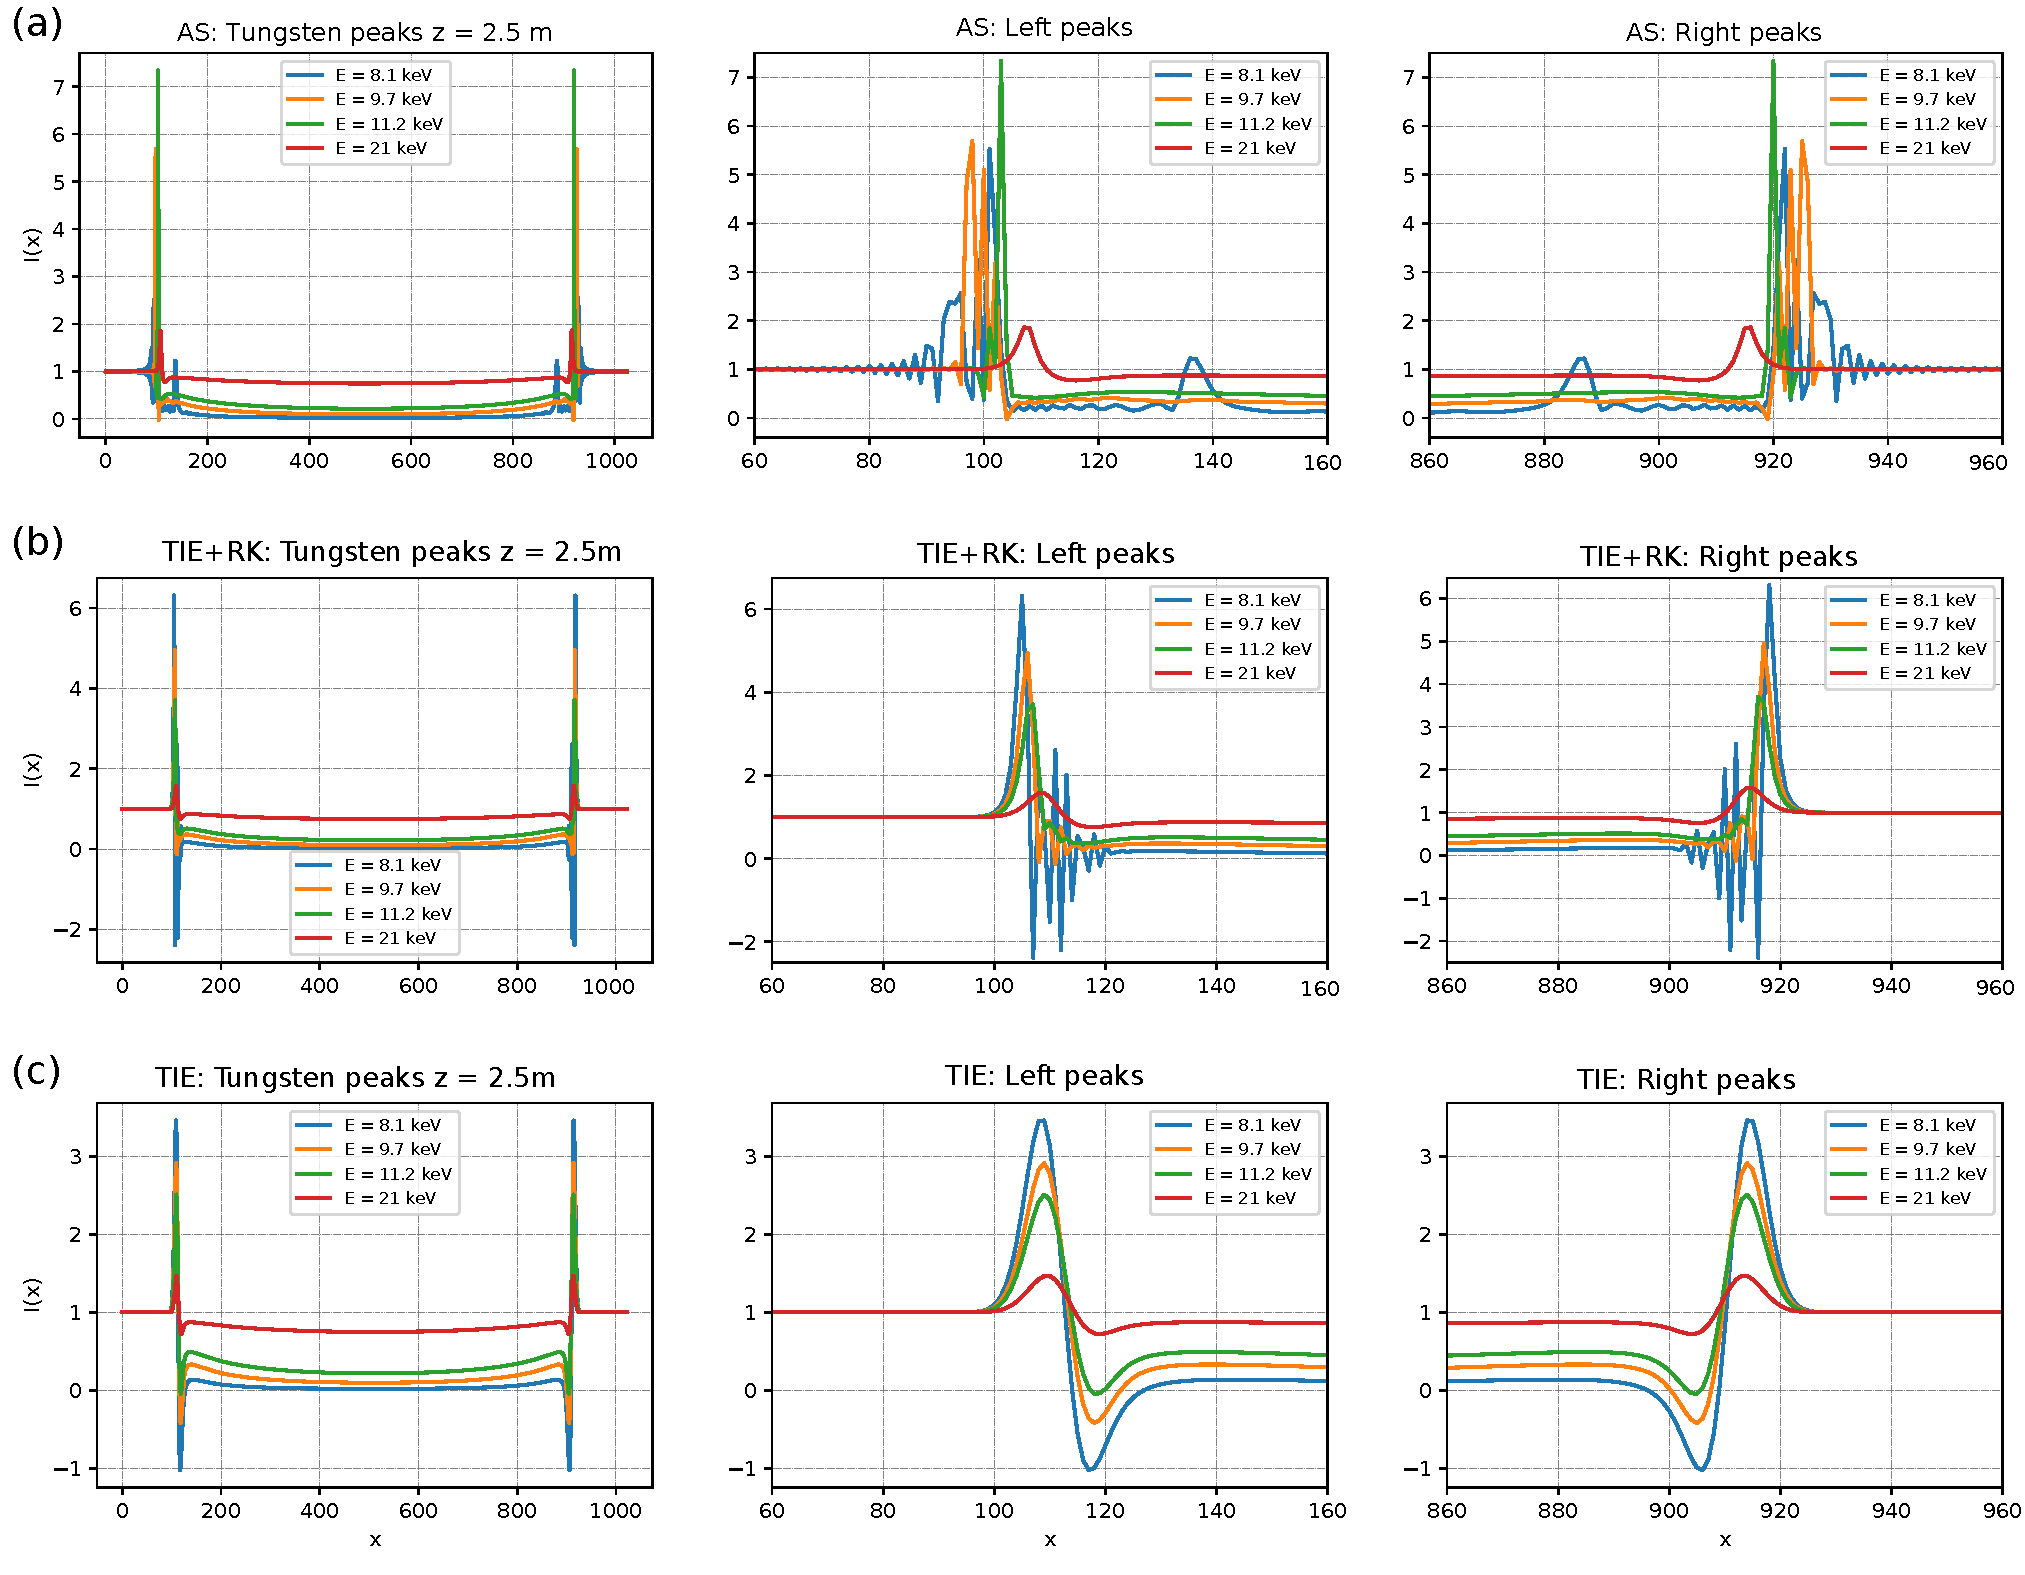
\includegraphics[width=1.1\linewidth]{AS_vs_TIE+RK_vs_TIE_1.pdf}
 \captionof{figure}{These nine plots demonstrate the behaviour of the phase contrast intensity fringes as a function of space and energy. The vertical axes represent intensity and the horizontal axes the pixel position, the different coloured curves represent the energy used to obtain the phase contrast intensity profile. Each row in this plot matrix represents the numerical method that was used to obtain the phase contrast plots, i.e. (a) Angular spectrum formulation (ASF), (b) transport-of-intensity equation implemented with fourth order-Runge-Kutta (TIE+RK), and (c) the conventional transport-of-intensity equation (TIE). The middle and right-most columns in this plot matrix display an amplified view of the left and right phase contrast fringes for each method respectively.}
\end{Figure}
As is clearly visible in figure \ref{fig:compare1}, each method produces different looking intensity profiles for each independent energy value. In the case of sub-figure (a) for the ASF, the numerical instability visible is much more pervasive than for the other two methods (i.e. (b) TIE+RK, (c) TIE). The ringing visible in the ASF plots only decreases when the energy value used is near the Bremsstrahlung peak of Tungsten. This is probably due to the construction of the ASF algorithm, since it is calculated in Fourier space. The nature of the ringing visible is probably due to the behaviour of Fourier sums undergoing large oscillations where they encounter jump discontinuities. The TIE+RK method also presents  ringing artefacts, but these are less exaggerated than the ASF. At the same time the TIE+RK method demonstrates similar intensity amplitudes to those shown in the ASF plots. Lastly the TIE method appears as the most numerically stable but it falls short from the phase contrast amplitudes achieved by the other two methods.

Regardless of the visible instability, the ASF method represents the most accurate solution to the phase contrast propagation problem. In figure \ref{fig:compare1} one can see that both the ASF and the TIE+RK methods have fringes that shift horizontally as the energy values increase, to see this effect more clearly see figure \ref{fig:compare2} below.
\begin{Figure}\label{fig:compare2}  
 \centering
  \hspace*{-0.9cm}
 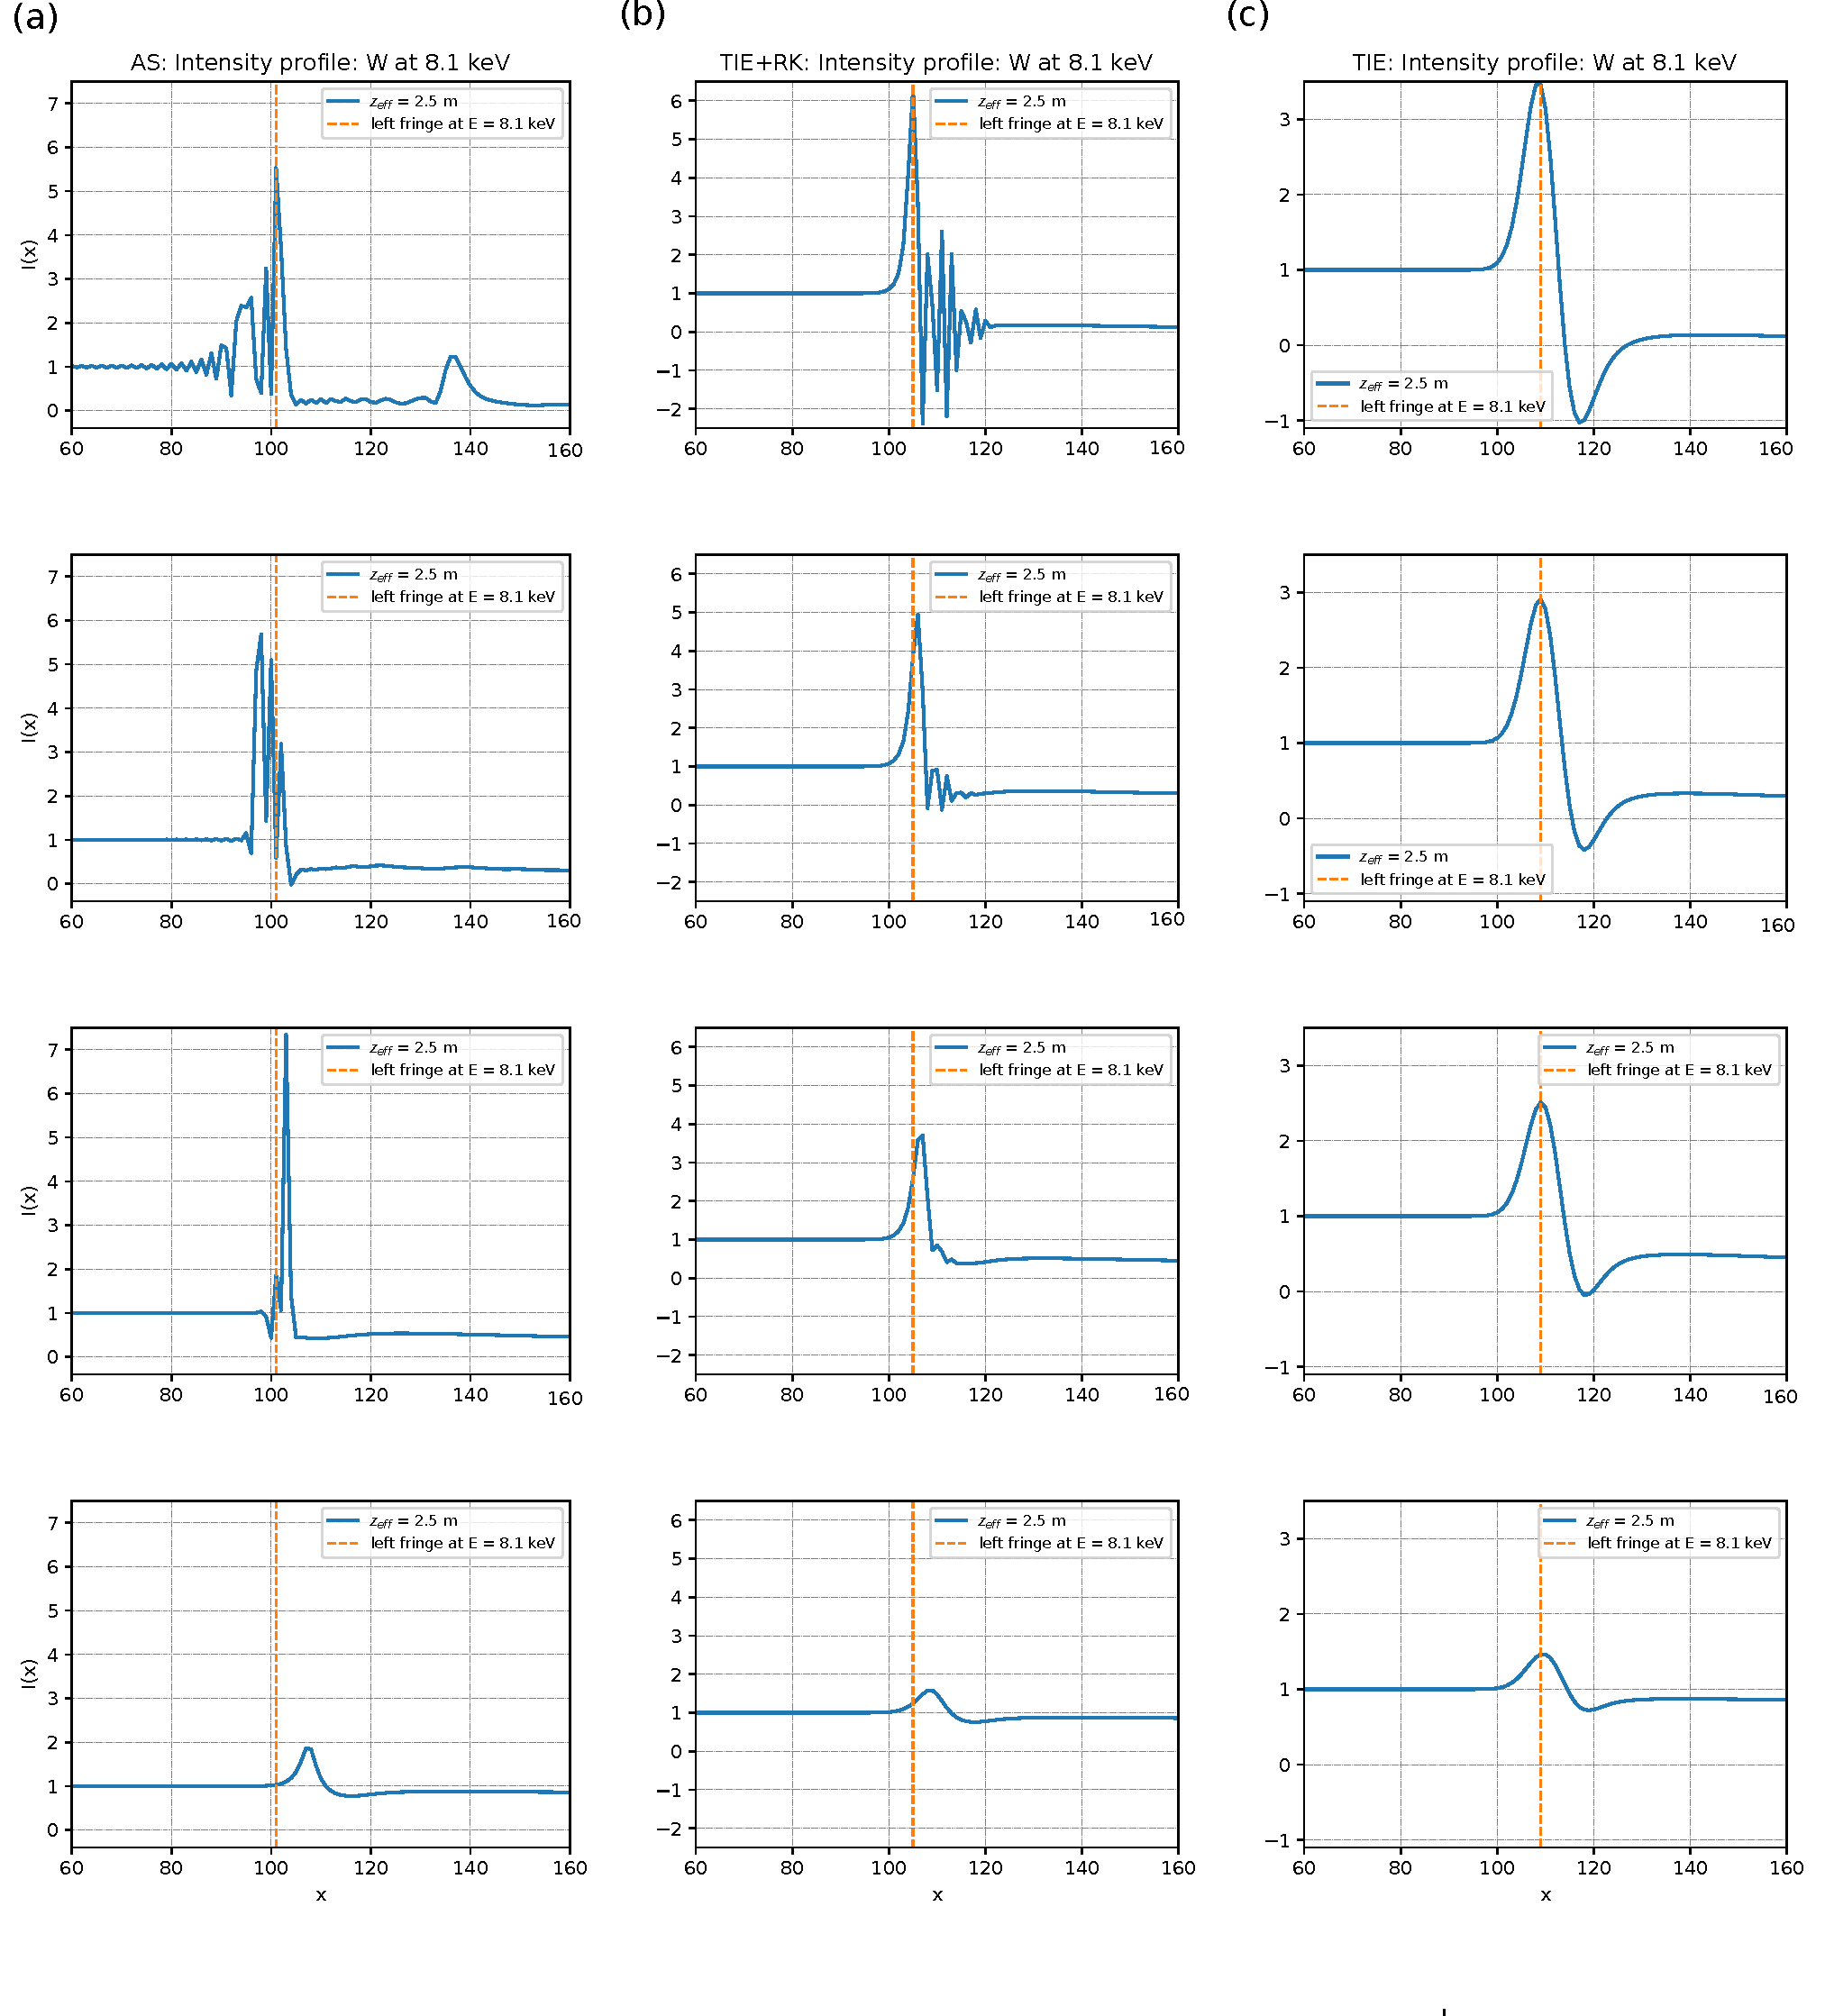
\includegraphics[width=1.1\linewidth]{AS_vs_TIE+RK_vs_TIE_2.pdf}
 \captionof{figure}{These twelve plots demonstrate the shifting behaviour of phase contrast fringes as a function of space and energy. This figure focuses solely on the \textbf{left} phase contrast fringe for each imaging method used in the fringe shifting simulations (see figure \ref{fig:compare1}). The plots' vertical axes represent intensity and the horizontal axes the pixel position. Each column in this matrix represents the method used to obtain the phase contrast intensity profiles (see sub-figures (a) ASF, (b) TIE+RK and (c) TIE). The sub-figures should be studied from top to bottom since the energy values used to obtain the phase contrast plots ranges from the top row at the lowest energy $E = 8.1$ keV, to $E = 9.7$ keV, and $E = 11.2$ keV and finally down to $E = 21$ keV in the last row. All phase contrast intensity profiles were obtained at a propagation distance $z = 2.5$ m. In order to easily observe the fringe shifting, I have included an orange vertical dashed line in each plot, this line marks the central position of the left phase contrast fringe at the lowest energy in the range $E = 8.1$ keV. This dashed line should be used as a reference of the horizontal fringe shifting for each method. The phase contrast fringes obtained using the ASF (visible in sub-figure (a)) move horizontally to the right approximately 6 pixels from the lowest energy to the highest energy in the range. The TIE+RK method (sub-figure (b)) shifts horizontally approximately 4 pixels in the same fashion as the ASF for the same energy range. Finally, the TIE method does not show a horizontal shift of fringes as a function of energy.}
\end{Figure}
MORE HERE $>>>>>>>>>>>>>>>>>>>$
%%%%%%%%%%%%%%%%%%%%%%%%%%%%%%%%%%%%%%%%%%%%%%%%%%%%%%%%%%%%%%%%%%%%%%%%%%%%%%%%%%%%%%%%%%%%%%%%%%%%%%%%%%%%%%%%%%%%%%%%%%%%%%%%%%%%%%%%%%%%%%%%%%%%%%%%%%%%%%%%%%%%%%%%%%%%%

\subsection{Verifying the problems with polychromatic spectra in the Lab}


MORE HERE $>>>>>>>>>>>>>>>>>>>$
%%%%%%%%%%%%%%%%%%%%%%%%%%%%%%%%%%%%%%%%%%%%%%%%%%%%%%%%%%%%%%%%%%%%%%%%%%%%%%%%%%%%%%%%%%%%%%%%%%%%%%%%%%%%%%%%%%%%%%%%%%%%%%%%%%%%%%%%%%%%%%%%%%%%%%%%%%%%%%%%%%%%%%%%%%%%%



\subsection{Simulating a single homogeneous cylinder}\label{Single cylinder}
The phase contrast images visible in figure \ref{fig:5} were obtained using a Fourier TIE method. This method was not able to simultaneously match the expected phase contrast peak height, at this energy while at the same time remaining fully stable. The parameters used to obtain this image were chosen to match a silver source, specifically the k-alpha 1 transition. The simulated material for this cylinder is water. As explained in section \ref{Brainz} the optical parameters for these simulations were obtained from the ``X-ray attenuation calculator".
\begin{Figure}\label{fig:5}
\centering
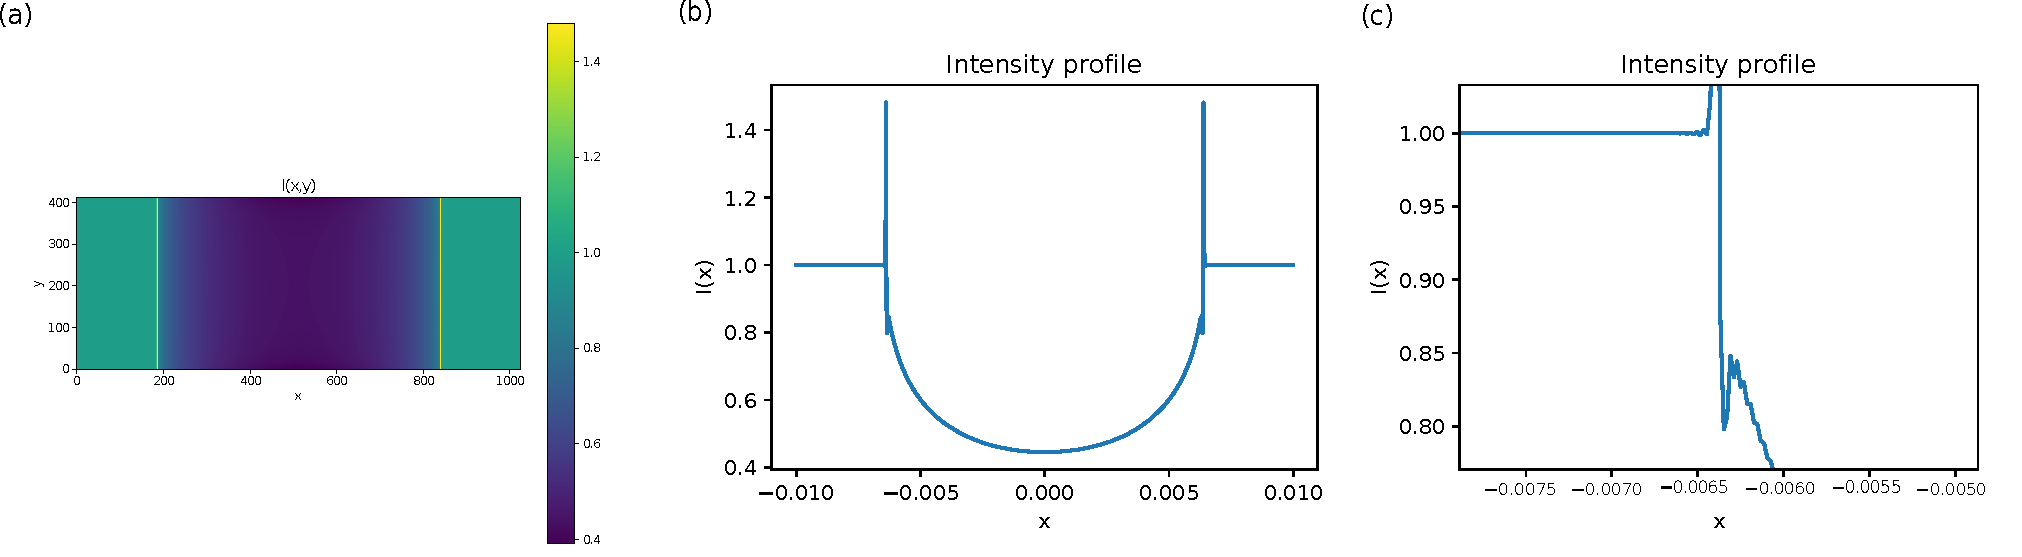
\includegraphics[width=\linewidth]{Fourier_intensity_profile.pdf}
\captionof{figure}{Phase contrast image (a), cross section (b), and enhanced view of (b) showing small ringing artefacts (instability)(c) obtained using the Fourier TIE method. The parameters used to obtain this image were an X-ray energy of $22.1629$ keV (corresponding to a Ag k-alpha 1 source), a refractive index decrement for the water cylinder of $\delta = 4.68141\times10^{-7}$ and an attenuation coefficient of $\mu = 64.38436~\mathrm{m^{-1}}$. The cylinder radius was $R = 6.375$ mm. The sigmoid function blurred $0.5$ pixels over the edge of the imaged cylinder. The propagation distance used was $z = 1$ m.}
\end{Figure}
From observing the results in figure \ref{fig:5}, I hypothesize that the underlying reason why my Fourier TIE method didn't work as expected was due to an effect known as Gibbs phenomenon, this effect occurs when the nth partial sum of a Fourier series undergoes large oscillations near regions with jump discontinuities\cite{Gibbs} (i.e. like the phase contrast fringes). Discovering that higher degree polynomial interpolation does not always improve accuracy was interesting and certainly unexpected.

The phase contrast images visible in figure \ref{fig:6} were obtained using a finite differences TIE and RK method. As can be seen here, the phase contrast peaks are much higher than the profile found using the Fourier method in figure \ref{fig:5}. The parameters used to obtain figure \ref{fig:6} were chosen to be identical to those used to obtain figure \ref{fig:5}, with the exception of the sigmoid blurring parameter, which was softer under the finite differences method.
\begin{Figure}\label{fig:6}  
\centering
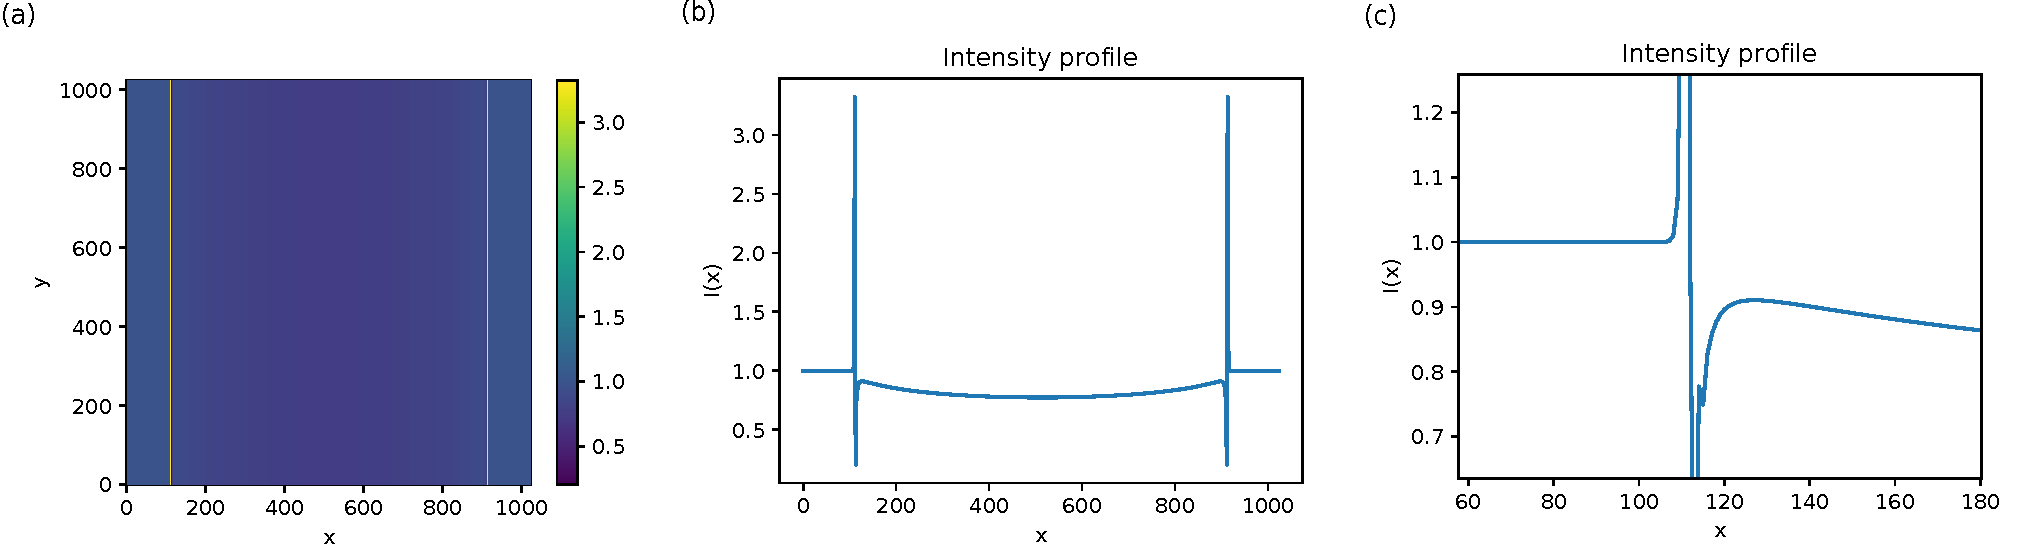
\includegraphics[width=\linewidth]{FD_intensity_profile.pdf}
\captionof{figure}{Phase contrast image and cross section. The parameters used to obtain this image were an X-ray energy of $22.1629$ keV (corresponding to a Ag k-alpha 1 source), a refractive index decrement for the water cylinder of $\delta = 4.68141\times 10^{-7}$ and an attenuation coefficient of  $\mu = 64.38436~\mathrm{m^{-1}}$. The cylinder radius was $R = 6.375$ mm. The sigmoid function blurred $0.14$ pixels over the edge of the imaged cylinder. The propagation distance used was $z = 1$ m. The apparent asymmetry of the two-dimensional phase contrast image is due to aliasing.}
\end{Figure}
This result presented an apparent improvement in the height of the expected phase contrast fringes when compared to the TIE method implemented by the xri library, and it lead me to explore the differences between my version of the TIE against other phase contrast propagation methods.
%%%%%%%%%%%%%%%%%%%%%%%%%%%%%%%%%%%%%%%%%%%%%%%%%%%%%%%%%%%%%%%%%%%%%%%%%%%%%%%%%%%%%%%%%%%%%%%%%%%%%%%%%%%%%%%%%%%%%%%%%%%%%%%%%%%%%%%%%%%%%%%%%%%%%%%%%%%%%%%%%%%%%%%%%%%%%

\subsection{Density difference test: water and ice}
As described in section \ref{2 cylinders}, to test if there is a density dependence in phase contrast, I first use a sample consisting of two cylinders with the outermost one made of water and the innermost one made of ice.
\begin{Figure}\label{fig:6}
\centering
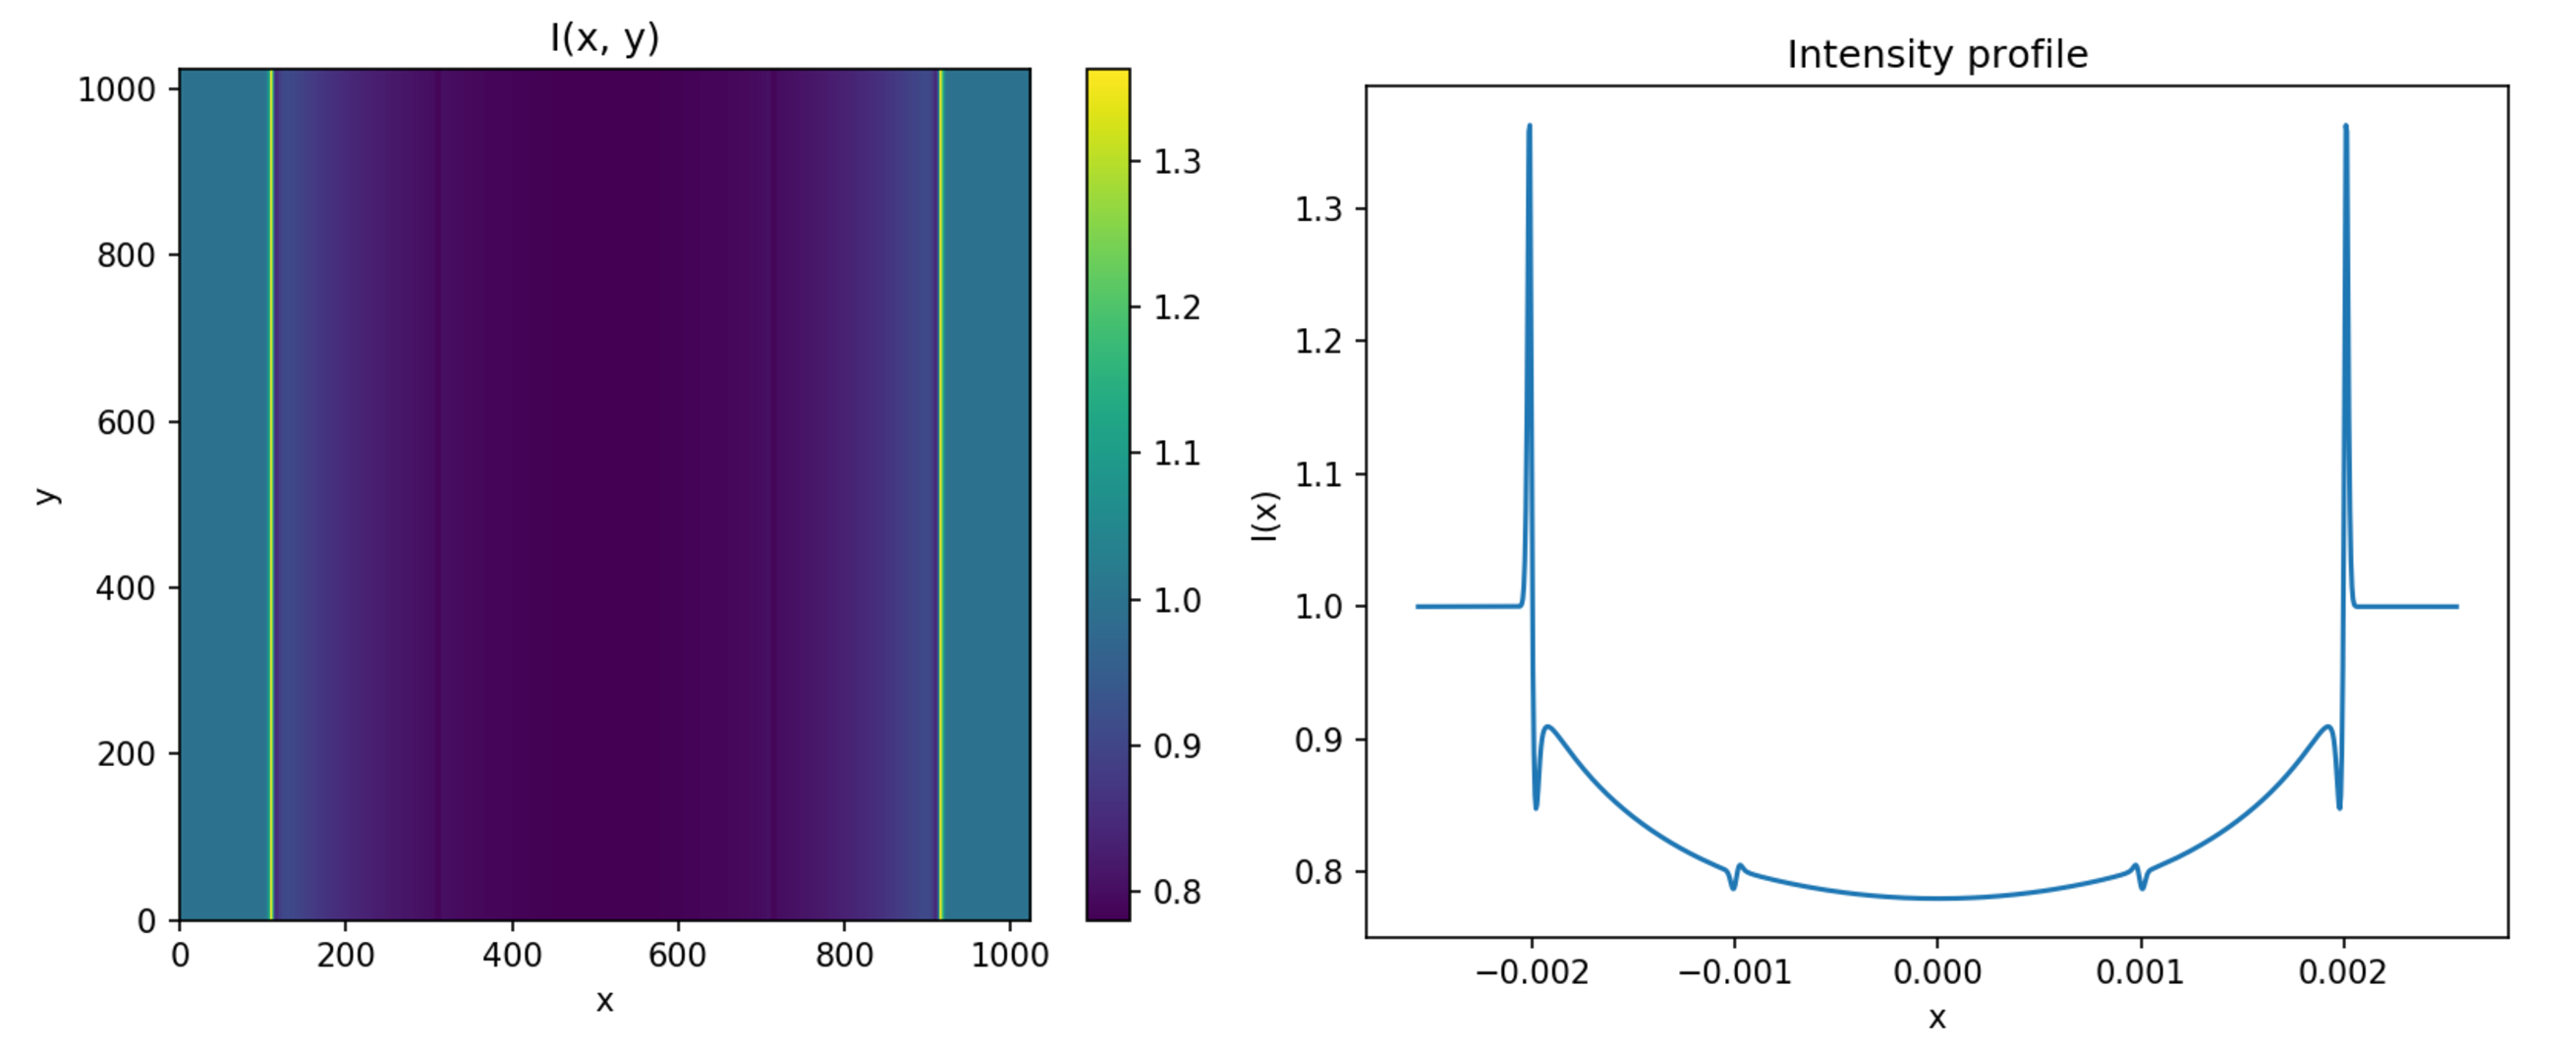
\includegraphics[width=\linewidth]{ice_water_AS.pdf}
\captionof{figure}{Phase contrast image and cross section obtained with the angular spectrum formulation method developed by the X-ray imaging group. The X-ray energy used in this simulation was $E = 22.1629$ keV. The water cylinder has a refractive index decrement $\delta_w = 4.69337\times10^{-7}$, the attenuation coefficient of water is $\mu_w = 64.55083~\mathrm{m^{-1}}$. The ice cylinder has a refractive index decrement $\delta_i = 4.31790\times10^{-7}$, and attenuation coefficient $\mu_i = 59.38677~\mathrm{m^{-1}}$. The density difference between these materials is $\Delta \rho = 0.08~\mathrm{g cm^{-3}}$. The cylinder's radii were $R_w = 2$mm and $R_i = 1$mm. The propagation distance used was $z = 2.5$ m.}
\end{Figure}
With the result in figure \ref{fig:6}. I demonstrate that any changes in material density throughout the imaged sample do affect the imaging process, and therefore the stability the propagation based imaging algorithm developed by Paganin et al. (2002) is actually dependent on the ratio of the differences in the refraction and attenuation coefficients $\Delta \delta$ and $\Delta \mu$ of the imaged materials.
In the following simulation, I take into account the apparatus parameters and the resolution of the detector used in the lab. I made this simulation to see whether or not we would be able to see the any small fringes in a real experiment. Using magnification factors we would use in the lab (i.e. $2.5$X and $4.0$X) and our photon detector dimensions I resized the spatial array boundaries to match those of the detector. I also scaled the pixel size to match the pixels in the photon detector. I did this so that the pixels in the object plane are adequately sized given the expected size of the pixels in the detector plane. I also calculated the effective propagation distance by dividing the simulation propagation distance by the desired magnification factor.
\begin{Figure}\label{fig:7}
\centering
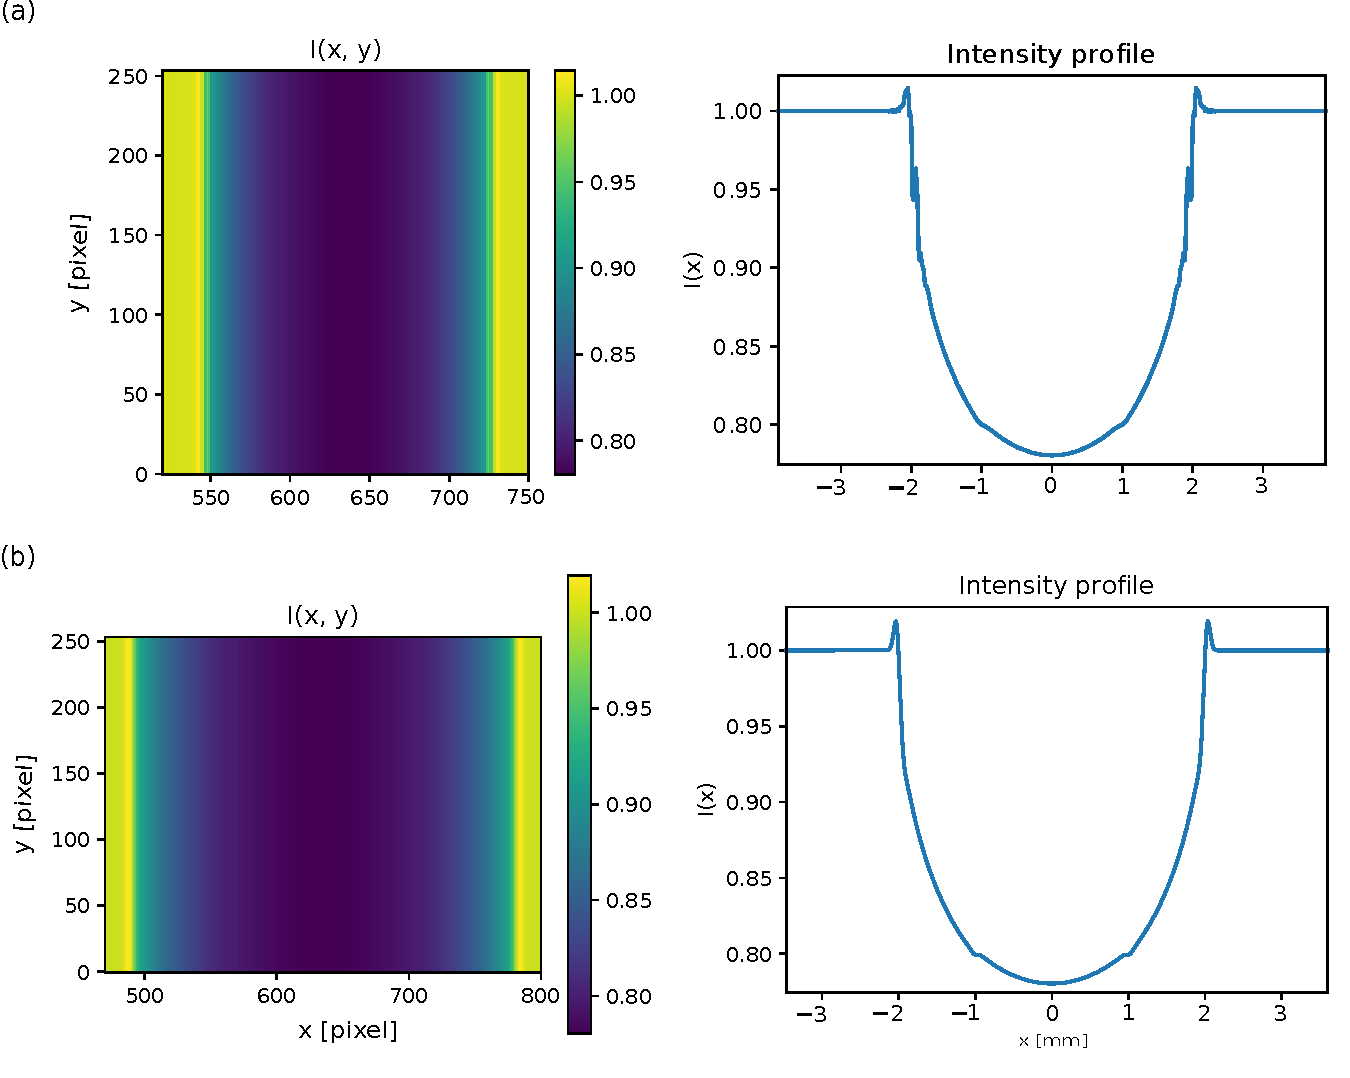
\includegraphics[width=\linewidth]{LAB_ice_water_AS_2_magnifications.pdf}
\captionof{figure}{Phase contrast cross sections were obtained with parameters equal to those in the simulation in figure \ref{fig:6}.}
\end{Figure}
The plan was to test these results experimentally, but given that the phase contrast fringes observable in figure \ref{fig:7} were so small, we decided against doing the experiment, since we would not observe much in a lab setting. 
\subsection{Density difference test: Grey matter and white matter}
To continue my tests of the importance of density in phase contrast, I assume in figure \ref{fig:8}, that grey and white matter have the same chemical compositions but distinct densities.
\begin{Figure}\label{fig:8}
\centering
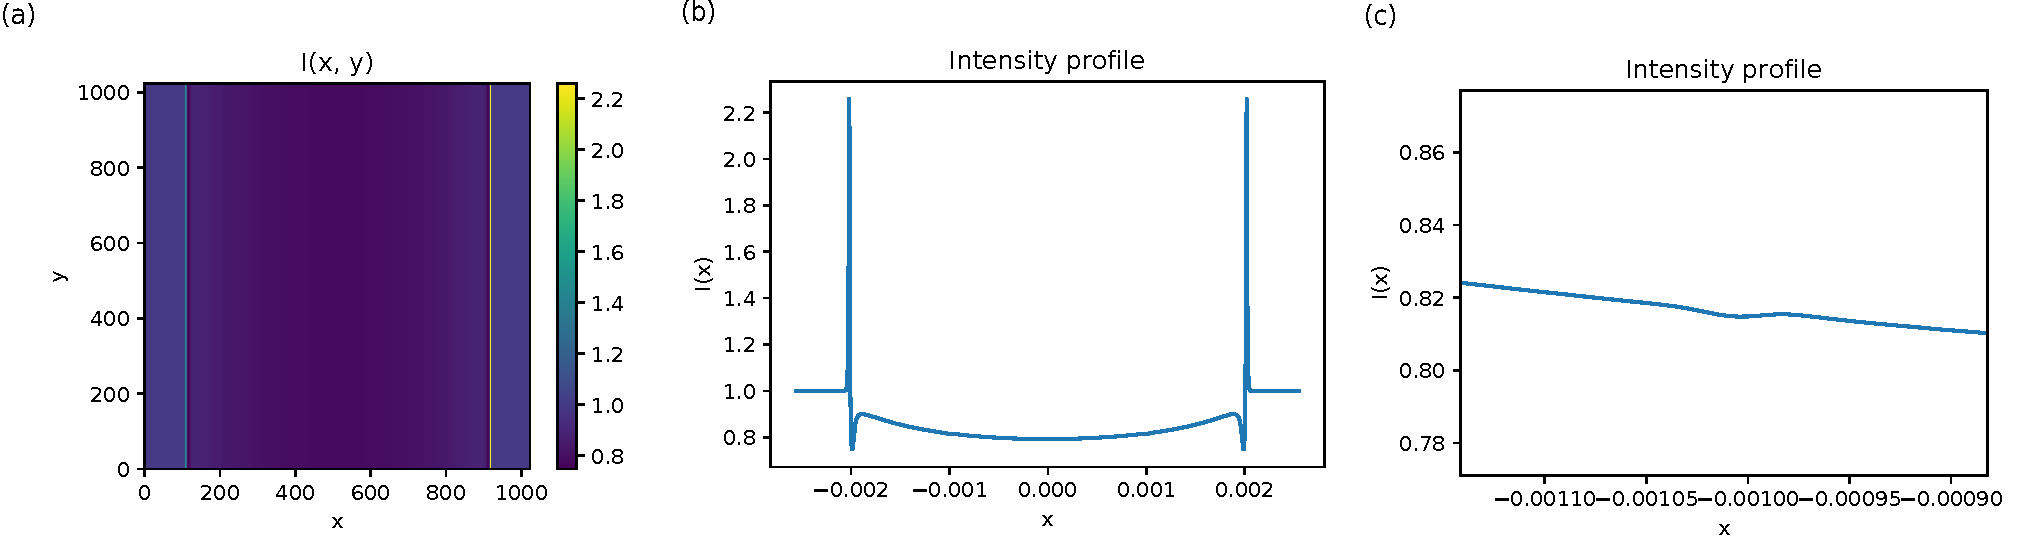
\includegraphics[width=\linewidth]{pessimistic_case.pdf}
\captionof{figure}{Phase contrast image (a), cross section (b), and enhanced view of one the inner cylinder phase contrast fringes (c) obtained with the angular spectrum formulation method as developed by the X-ray imaging group. In (c) it can be seen that the phase contrast fringes from the inner cylinder are extremely small but can still be observed when the image in (b) is amplified enough. The X-ray energy is $E = 24$ keV. The grey matter cylinder has a refractive index decrement $\delta_{\mathrm{GM}} = 4.1345\times10^{-7}$, and the attenuation coefficient of grey matter is $\mu_{\mathrm{GM}} = 58.2978~\mathrm{m^{-1}}$. The white matter cylinder has a refractive index decrement $\delta_{\mathrm{WM}} = 411.87\times10^{-7}$ and its attenuation coefficient $\mu_{\mathrm{WM}}= 58.0747~\mathrm{m^{-1}}$. The density difference between these materials is $\Delta \rho = 0.004~\mathrm{g cm^{-3}}$\cite{ITIS}. The cylinders' radii were $R_{\mathrm{GM}} = 2$ mm and $R_{\mathrm{WM}} = 1$ mm. The propagation distance used was $z = 2.5$ m.}
\end{Figure}
My simulations demonstrate that even a small density difference like the one seen in \ref{fig:8} can produce phase contrast fringes. Nevertheless, my simulations only consider perfect data, therefore the fringes would be too small to see using real sample materials in a lab experiment.

%%%%%%%%%%%%%%%%%%%%%%%%%%%%%%%%%%%%%%%%%%%%%%%%%%%%%%%%%%%%%%%%%%%%%%%%%%%%%%%%%%%%%%%%%%%%%%%%%%%%%%%%%%%%%%%%%%%%%%%%%%%%%%%%%%%%%%%%%%%%%%%%%%%%%%%%%%%%%%%%%%%%%%%%%%%%%

\subsection{Chemical difference test: Grey matter and white matter}
Here I continue the tests of phase contrast for brain materials. As opposed to the simulation in figure \ref{fig:8}, the simulation in figure \ref{fig:9} assumes that grey and white matter are different chemically. This condition returns clear fringes for both outer and inner cylinders. This simulation likely represents a more realistic output then \ref{fig:8}
given that there are likely chemical differences between the materials in a real brain.
\begin{Figure}\label{fig:9}
\centering
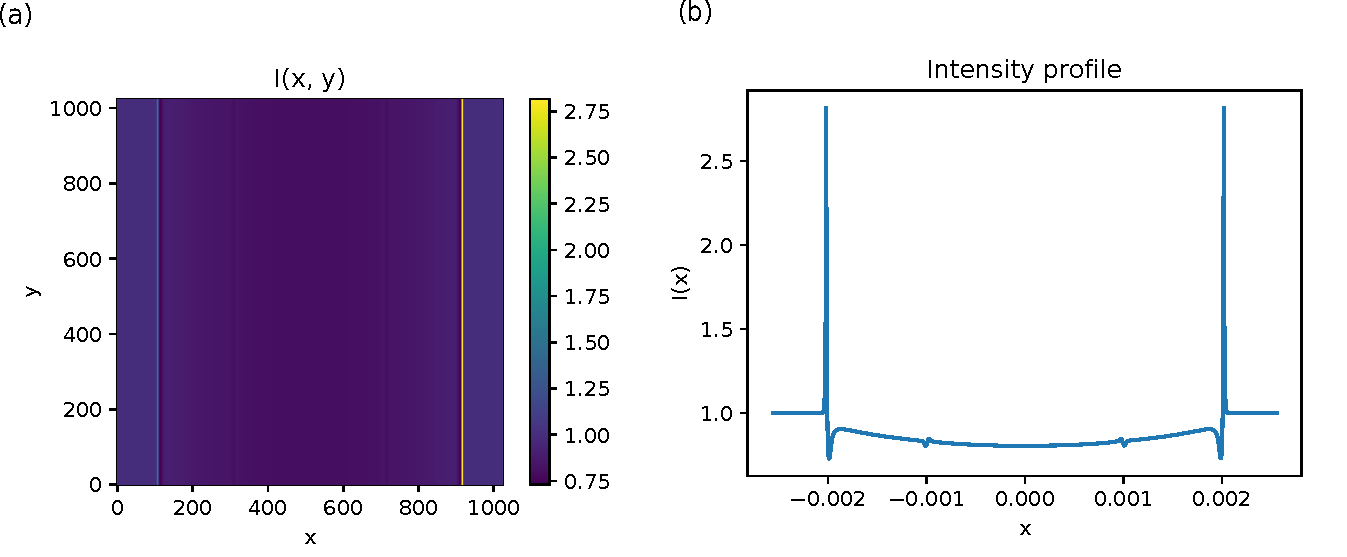
\includegraphics[width=\linewidth]{optimistic_case.pdf}
\captionof{figure}{Phase contrast image and phase contrast cross section obtained with the angular spectrum formulation method developed by the X-ray imaging group. The X-ray energy used in this simulation was $E = 24$keV. The grey matter cylinder has a refractive index decrement $\delta_{\mathrm{GM}} = 4.591\times10^{-7}$, the attenuation coefficient of grey matter is $\mu_{\mathrm{GM}} = 52\mathrm{m^{-1}}$\cite{Linda}. The white matter cylinder has a refractive index decrement $\delta_{\mathrm{WM}} = 4.2631\times10^{-7}$ and attenuation coefficient $\mu_{\mathrm{WM}}= 56~\mathrm{m^{-1}}$\cite{Linda}. The cylinders' radii were $R_{\mathrm{GM}} = 2$ mm and $R_{\mathrm{WM}} = 1$ mm. The propagation distance used was $z = 2.5$m.}
\end{Figure}
%%%%%%%%%%%%%%%%%%%%%%%%%%%%%%%%%%%%%%%%%%%%%%%%%%%%%%%%%%%%%%%%%%%%%%%%%%%%%%%%%%%%%%%%%%%%%%%%%%%%%%%%%%%%%%%%%%%%%%%%%%%%%%%%%%%%%%%%%%%%%%%%%%%%%%%%%%%%%%%%%%%%%%%%%%%%%
MORE HERE $>>>>>>>>>>>>>>>>>>>$

\chapter{Conclusion}\label{Conclusion}
MORE HERE $>>>>>>>>>>>>>>>>>>>$
%%%%%%%%%%%%%%%%%%%%%%%%%%%%%%%%%%%%%%%%%%%%%%%%%%%%%%%%%%%%%%%%%%%%%%%%%%%%%%%%%%%%%%%%%%%%%%%%%%%%%%%%%%%%%%%%%%%%%%%%%%%%%%%%%%%%%%%%%%%%%%%%%%%%%%%%%%%%%%%%%%%%%%%%%%%%%


\chapter{Acknowledgements}\label{Acknowledgements}

I want to thank my supervisor Marcus for guiding me through the semester with great suggestions and lots of encouragement. I always enjoyed our talks about physics and other topics. I also want to thank our research group members for being so welcoming and, specifically to Linda for helping me with my writing, and to James for helping during my experiment. Lastly, I want to thank my partner Chris for being an endless source of inspiration, helpful advice and for all our interesting rants and discussions.  
%%%%%%%%%%%%%%%%%%%%%%%%%%%%%%%%%%%%%%%%%%%%%%%%%%%%%%%%%%%%%%%%%%%%%%%%%%%%%%%%%%%%%%%%%%%%%%%%%%%%%%%%%%%%%%%%%%%%%%%%%%%%%%%%%%%%%%%%%%%%%%%%%%%%%%%%%%%%%%%%%%%%%%%%%%%%%

\chapter{Appendix}\label{Appendix}
\section{Exploring phase retrieval with TIE+RK}\label{Aborted}
MORE HERE $>>>>>>>>>>>>>>>>>>>$
\subsection{Methods}
MORE HERE $>>>>>>>>>>>>>>>>>>>$
%%%%%%%%%%%%%%%%%%%%%%%%%%%%%%%%%%%%%%%%%%%%%%%%%%%%%%%%%%%%%%%%%%%%%%%%%%%%%%%%%%%%%%%%%%%%%%%%%%%%%%%%%%%%%%%%%%%%%%%%%%%%%%%%%%%%%%%%%%%%%%%%%%%%%%%%%%%%%%%%%%%%%%%%%%%%%

\subsection{Results}
MORE HERE $>>>>>>>>>>>>>>>>>>>$
% \begin{Figure}
% \centering
% \includegraphics[width=\linewidth]{phase_retrieval.pdf}
% \captionof{figure}{}
% \end{Figure}
MORE HERE $>>>>>>>>>>>>>>>>>>>$

% can we use TIE+RK in phase retrieval?
% Can TIE+RK be used for phase retrieval?

 % no one has successfully developed a phase retrieval algorithm based on the AS, but there are many such solutions using the TIE. 

 % One example is attached where the authors did use higher order terms instead of the finite difference approximation to improve phase retrieval, but it required multiple images to be acquired. This is a problem for X-ray imaging as it will increase the radiation dose. David Paganin's single image algorithm (attached) is ideal as it is noise robust and only requires a single exposure, but is based on the TIE with the finite difference approximation.

 % I don't know that the RK approach can help with phase retrieval, but I'd certainly like to think about that more.

MORE HERE $>>>>>>>>>>>>>>>>>>>$
%%%%%%%%%%%%%%%%%%%%%%%%%%%%%%%%%%%%%%%%%%%%%%%%%%%%%%%%%%%%%%%%%%%%%%%%%%%%%%%%%%%%%%%%%%%%%%%%%%%%%%%%%%%%%%%%%%%%%%%%%%%%%%%%%%%%%%%%%%%%%%%%%%%%%%%%%%%%%%%%%%%%%%%%%%%%%

\bibliography{mybib}
\bibliographystyle{unsrt}
\end{document}